%\documentclass[pldi]{sigplanconf-pldi16}
\documentclass[10pt]{sigplanconf}
%\usepackage{usenix,epsfig,endnotes}

%\usepackage{epsfig,endnotes}
% standard LaTeX packages
%\usepackage{changebar}
\usepackage[normalem]{ulem}
\usepackage{balance}
\usepackage{alltt}
\usepackage{amsmath}
\usepackage{balance}
\usepackage{booktabs}
\usepackage{fixltx2e}
\usepackage{graphicx}
\usepackage{boxedminipage}
\usepackage{hyperref}
\usepackage{nicefrac}
\usepackage{subfig}
%\usepackage{xcolor}
\usepackage{setspace}
\usepackage{xspace}
\usepackage{multirow}
\usepackage{colortbl}
\usepackage{amsfonts} 
\usepackage{blindtext}
\usepackage{chngpage}
\usepackage{listings}
\usepackage{color}
\usepackage[dvipsnames]{xcolor}
\usepackage{mathtools}
\usepackage{amssymb}
\usepackage{pifont}
\usepackage[numbers,sort&compress,square]{natbib}

\usepackage{wrapfig}
%% Golang definition for listings
%% http://github.io/julienc91/lstlistings-golang
%%
\RequirePackage{listings}

\lstdefinelanguage{Golang}%
  {morekeywords=[1]{package,import,func,type,struct,return,defer,panic,%
     recover,select,var,const,iota,},%
   morekeywords=[2]{string,uint,uint8,uint16,uint32,uint64,int,int8,int16,%
     int32,int64,bool,float32,float64,complex64,complex128,byte,rune,uintptr,%
     error,interface},%
   morekeywords=[3]{map,slice,make,new,nil,len,cap,copy,close,true,false,%
     delete,append,real,imag,complex,chan,},%
   morekeywords=[4]{for,break,continue,range,goto,switch,case,fallthrough,if,%
     else,default,},%
   morekeywords=[5]{Println,Printf,Error,Print,},%
   sensitive=true,%
   morecomment=[l]{//},%
   morecomment=[s]{/*}{*/},%
   morestring=[b]',%
   morestring=[b]",%
   morestring=[s]{`}{`},%
   }

\lstset{
  basicstyle=\tiny,
  columns=fullflexible,
  numbersep=5pt,
  numberstyle=\tiny,
  showstringspaces=false,
  escapeinside={/*@}{@*/},
  belowcaptionskip=1\baselineskip,
  language=Golang,
  showstringspaces=true,
  basicstyle=\scriptsize\ttfamily,
  keywordstyle=\bfseries\color{Cerulean},
  commentstyle=\itshape\color{PineGreen},
  identifierstyle=\color{Violet},
  stringstyle=\color{Brown},
  stepnumber=1,                    % the step between two line-numbers. If it's 1, each line will be numbered
  firstnumber=1,
  numberfirstline=true,
  numbers=left
}

%\pgfplotstableset{
%    color cells/.style={
%        col sep=comma,
%        string type,
%        postproc cell content/.code={%
%                \pgfkeysalso{@cell content=\rule{0cm}{2.4ex}\cellcolor{black!##10}\pgfmathtruncatemacro\number{##1}\ifnum\number>5\color{white}\fi##1}%
%                },
%        columns/x/.style={
%            column name={},
%            postproc cell content/.code={}
%        }
%    }
%}


%\makeatletter
%\def\@copyrightspace{\relax}
%\makeatother

\captionsetup{format=default, font=bf}


\newcommand*{\Scale}[2][4]{\scalebox{#1}{$#2$}}%
%\newcommand{\comment}[1]{{}}



%% taken from unknown.sty
%\DeclareCaptionType{copyrightbox}

\sloppy

\input macros.tex

\begin{document}


\twocolumn[
\begin{@twocolumnfalse}
\begin{center}
{\Large\bf Protocol Dialect Generation with State Machine Variation}
\end{center}
%\smallskip
%\vspace{-0.2in}
%\begin{center}
%Xiaoyu Liu$\ast$,
%Linhai Song$\dagger$,
%Yiying Zhang$\ast$ \\
%$\ast$ Purdue University, $\dagger$ Pennsylvania State University
%\end{center}

\bigskip
\end{@twocolumnfalse}
]



%\theoremstyle{definition}
%\newtheorem{definition}{Definition}[section]

%\begin{abstract}
%\input{section/0_abstract}
%\end{abstract}

\def\ie{\emph{i.e.}}
\def\eg{\emph{e.g.}}

\newcommand{\hpad}[0]{\hspace*{\fill}}

\newcommand{\Thrust}[1]{\hyperref[sec:thrust-#1]{Thrust #1}}
\newcommand{\Code}[1]{\lstinline{#1}}


\section{Introduction} 
\label{sec:intro}

% Background

To facilitate communication with external entities and coordination with
internal operations, private networks (\eg, data centers and industrial control
networks) run a wide range of conventional protocols (\eg, Secure Socket Layer
\texttt{SSL}~\citep{tls-wiki} and Lightweight Directory Access Protocol 
\texttt{LDAP}~\citep{LDAP}). 
As a result, they are typically vulnerable to not only the security loopholes
residing in the protocol but also the DDoS attackes resulting from protocol
abuses~\citep{LDAP-abuse1,LDAP-abuse2,NTP-abuse}.

To safeguard such private networks, network administrators typically adopt
firewalls~\citep{firewall} to detect intruders. 
However, they provide only limited security
guarantee to the daily operations in private networks~\citep{firewall-limitation}. 
On the one hand, this is
because private networks use public protocols both internally and externally,
and it is sometimes difficult for firewalls to characterize the abnormal
behaviors of public protocols. On the other hand, this is due to the fact that
firewalls are typically ineffective when the attack is launched internally.

From the perspective of network defenses, we believe the best practice for
addesssing this issue is to customize protocols so that they can be used for
internal and external communications differently. By customizing the dialog of
\texttt{LDAP} protocol and using it only for internal communications or
operations, for example, we could augment a private network with the ability to
drop off the internal packets different from the customization, making the
network naturally resistant to the DDoS reflection attack resulting from the
abuse of conventional \texttt{LDAP}. However, protocol customization could be
extrememely difficult and time-consuming. Given a complicated communication
protocol, it generally requires a software developer putting a large amount of
manual efforts to ensure his customization does not introduce logic
incorrectness nor runtime failures.

% Our research

Inspired by this, we propose a protocol customization techniques to diversify
protocols commonly adopted in private networks. More specifically, we plan to
design and develop a full stack of technical approaches that could automate
protocol modification and thus generate various dialogs for a target protocol.
Since a network protocol typically can be modeled as a set of finite state
machines involved in communication, technically speaking, we will first develop
an effective mechanism to identify the implemenation pertaining to the state
machines responsible for message exchanging. Then, we will utilize and design
static program analysis techniques to analyze protocol implementations,  extract
state machines and fully restore the communication dialogs they involved.

Since the ultimate goal of this research project is to generate various protocol
dialogs, we will further explore various approaches to mutate a communication
dialog and identify those mutation strategies that do not jeoparidize the
validity of a target protocol. We intend to implement the strategies  identified
through an automated tool. Thus, we will also design and develop various program
synthesis techniques. To be more specific, we will research how to utilize
various program analysis techniques to perform code removal as well as code
generation. In the rest of the proposal, we will mainly descirbe how we plan to
design and develop these technical mechanisms, and discuss the technical
challenges we have to address. In addition, we introduce the research works that
we have already conducted.






% Private network always becomes the target of an attack, which extrernal
% intruders probe the networks and attempts to exploit or conduct Dos. To
% address this problem, traditional solution rely upon firewall to detect
% intruder. While it is effective, it does not guarantte to block external
% intrusion because the limitation.  Network intrusion largely rely upon the
% signatures. But some attack does not have signatures. Therefore, it sometimes
% fails to flag a intrusion or mistakenly tag a legit connect as malicious.

% To address this issue, we believe one solution to safegaurd private network is
% to use private protocol because (1) identifying intrusion detection in a
% private network without firewall (2) could potentially reduce the code bases
% -- tightening constraint -- making software resistant to known vulnerabilities
% (3) could reduce the network overhead -- merging network traffic. However,
% customizing a protocol to a private dialog needs a lot of manual efforts and a
% large amount of expertises. To make it worse, it is difficult to ensure the
% customized protocol is still valid.






% \newpage

\begin{table}[t]
\centering
 \begin{tabular}{|c c l|} 
 \hline
 Software & LoC & Description \\  
 \hline\hline
 \multicolumn{3}{|c|}{\textbf{Network Middelware Programs}}\\
 \texttt{PRADS-0.2}             & 28,083      & IDS \\ 
 \texttt{snort-2.9.9}           & 336,082     & IDS \\ 
 \texttt{haproxy-1.7.9}         & 97,278      & Load Balancer \\ 
 \texttt{Openvpn-2.4.3}         & 120,018     & Open-source VPN \\
 \texttt{Squid-2.5.27}          & 291,433     & Web Cache\\
 \hline\hline
 \multicolumn{3}{|c|}{\textbf{Interet of Things Applications}}\\
 \texttt{midilib} & 3,042 & MIDI protocol library \\ 
 \texttt{libmodbus} & 5,567 & A serial communications protocol \\ 
 \texttt{Eclipse Paho-mqtt} & 30,406 & Open and standard messaging protocols for IoT \\ 
 \texttt{Eclipse Paho-mos} & 33,429 & An open source message broker \\ 
 \texttt{open62541} & 37,020 & An open source implementation of OPC UA \\ 
 \texttt{Eclipse Wakaama} & 20,480 & Open Mobile Alliance's LightWeight M2M protocol \\ 
 \texttt{AwaLWM2M} & 106,319 & OMA Lightweight M2M protocol \\ 
 \texttt{mbed TLS} & 77,727 & SSL Library mbed TLS \\ 
 \texttt{OpenSSL} & 516,007 & Toolkit for the Transport Layer Security \\ 
 \texttt{dnp3} & 141,555 & Distributed Network Protocol \\ 
 \texttt{libcoap} & 35,125 & C-Implementation of CoAP \\ 
 \texttt{OpENer} & 20,103 & An EtherNet/IP stack for I/O adapter devices \\ 
 \hline
 \end{tabular}
\caption {A list of protocol implementations covering complicated network
middleware and lightweight IoT applications. Note that LoC indicates the lines
of code.}
\label{tab:software}
\end{table}


\section{Extracting Finite State Machines pertaining to Target Protocol}
\label{sec:subsetting}

As is discussed in the section above, the ultimate goal of this research project
is to generate customized dialects for protocols. To achieve this, we must
design and develop a mechanism to extract state machines pertaining to
protocols. In this section, we first discuss the challenges of protocol
extraction. Then, we describe our preliminary exploration followed by our
proposed techniques.

\subsection{Challenges}

From the perspective of software development, one can implement a
set of protocols in different forms. For example, a software developer may make
two protocols sharing the same code fragments or implement them separately or
use different data structures to define the state machines pertaining to
corresponding protocols. As such, the challenges of this research task include
(1) identifying the common patterns of protocol implementations, (2) pinpointing
the states pertaining to a protocol and (3) tracking down the state machines
pertaining to target protocols. In the following session, we discuss how we
intend to tackle these challenges.

\subsection{Preliminary Exploration}
\label{sec:task1:obs}

\begin{wraptable}{r}{.38\textwidth}
\centering
\begin{tabular}{c}
\hspace{12pt}

\begin{lstlisting}  
typedef enum {
    WORK_ERROR,
    WORK_FINISHED_STOP,
    WORK_FINISHED_CONTINUE,
    WORK_MORE_A,
    WORK_MORE_B,
    WORK_MORE_C
} WORK_STATE;
\end{lstlisting}

\end{tabular}
\caption{An enumeration type containing 6 integral constants indicating all the states pertaining to a
transmission protocol in \texttt{OpenSSL}.}
\label{code:enum}
\end{wraptable} 

To tackle these challenges, we must understand how developers typically
implement protocols in software. In this project, we therefore plan to start
with studying the implementation of various protocols. As our preliminary
exploration, we manually investigated the protocol implementation in software
specified in Table~\ref{tab:software}. As we can observe in the table, the
software we studied covers not only complicated network middleware like
\texttt{HAProxy} and \texttt{OpenVPN} but also lightweight IoT applications such
as \texttt{midilib} and \texttt{AwaLWM2M}. In the following, we summarize the
key observations obtained from this preliminary manual study.

Based on our manual study across all the software in Table~\ref{tab:software},
we first observe that a stateful protocol is typically implemented either in a
loop or a call back function. For example, Table~\ref{code:midilib} shows a
transmission protocol that is implemented in an infinite loop~\footnote{We consider 
a loop not iterating a specified number of times as an infinite loop.}. 
We believe that
this observation can be generalized, and an infinite loop or a call back can be
used for identifying a protocol implementation. This is due to the fact that a
stateful protocol is a finite state machine that needs to retain session
information and keep alive during program execution, and the best practice of
implementing such a protocol is through an infinite loop or a call back
function.

In addition to using a loop or a call back to implement a stateful protocol, we
observe that software developers typically utilize the enumeration data type
(\texttt{enum}) to define the states pertaining to a state machine. As is shown
in Table~\ref{code:enum}, for example, \texttt{WORK\_STATE} is an enumeration
type, which consists of 6 integral constants indicating all the states
pertaining to a transmission protocol in \texttt{OpenSSL}.

From our manual investigation,  we also observed that enumeration type is not
always used for the definition of protocol states nor the only data type that
implements states pertaining to a protocol. However, we believe it can be
potentially used to facilitate the identification of variables that implement
the states of a protocol. In the following section, we will discuss how we
intend to do so by taking this observation.

\begin{wraptable}{r}{.38\textwidth}
\centering
\begin{tabular}{c}
\hspace{12pt}

\begin{lstlisting}  
/* midifile.c */
bool midiReadGetNextMessage(const MIDI_FILE *_pMF, int iTrack, MIDI_MSG *pMsg) {
	if ((pMsg->iType & 0xf0) != 0xf0)
		...
}

/* m2rtttl.c */
MIDI_MSG msg; // MIDI_MSG is a struct type
... 
while(midiReadGetNextMessage(mf, i, &msg)) {
	...
	if (iCurrPlayingNote==msg.MsgData.NoteOff.iNote) {
		...
		iCurrPlayingNote = -1;
		...
	}
	...
}
\end{lstlisting}

\end{tabular}
\caption{The code fragments indicating the implementation of midi protocol.}
\label{code:midilib}
\end{wraptable} 

Last but not least, we observe software developers tend to use composite data
type to define the data packets exchanged between communication entities.
Typically, this kind of data structures is involved in bitwise operations and
tied to function calls pertaining to message read and write. For example, the
\texttt{midi} protocol defines data packet \texttt{msg} in struct
\texttt{MIDI\_MSG}. As is shown in Table~\ref{code:midilib}, software developers
tie it to message read function \texttt{midiReadGetNextMessage} and utilize
bitwise operations (see \texttt{lines 3}) to examine the values in this data
structure. In this project, we plan to leverage this observation to facilitate
the identification of the data structure pertaining to the data packets of the
target protocols. Though it might introduce some false positives or false
negatives, we believe this observation is relatively reliable for data structure
identification for the following reason. In most protocols, the information must
be packed into the data block without leaving any unused bits between the
fields. To make the best use of a data packet, the best practice is to make
extensive use of bitwise and shift operators to take the information values and
pack them into the payload being transmitted. In the following, we will further
discuss how we intend to utilize the key observations above to perform protocol
extraction or in other words the state machines pertaining to protocols residing
in the target software.

\subsection{Proposed Techniques}

Following the observations above, we will design and develop a series of
technical approaches to (1) identify the code fragments representing protocol
implementation, (2) pinpoint the variables that
implement the states of protocols, and (3) track down the state transitions and
thus construct the finite state machines pertaining to the protocols in target
software. In addition, we will explore, design and develop technical approaches
to refine the state machines, making sure the state machines extracted truly
represent that specified in a target protocol. In the following section, we
describe and discuss how we plan to design and develop these techniques in more
details.

\subsubsection{Research Task 1: Identifying Code Fragments Pertaining to
Protocol Implementation}
\label{subsec:rt1}

As is described above, the protocol implementation is typically associated with
an infinite loop or a call back function. In this project, we intend to use this
pattern to narrow down the implementation of a protocol in source code. In
particular, we plan to perform an exhaustive search on the code base of target
software, extract all the infinite loop and call back functions and treat these
as the candidates of protocol implementation. As is mentioned above, this
candidate set however may contain implementation not relevant to protocols.
Therefore, we will further introduce some heuristics to reduce false positives
and negatives introduced by this trivial approach.

Intuition suggests that the implementation of a stateful protocol must contain
the state variables, and the transitions between states must depend upon the
data packets transmitted. As a result, going beyond simply identifying infinite
loops and call back functions, our technique will examine if the state variable
is included in the candidate code fragments. In addition, we augment our
protocol identification technique with the ability to examine if state
transitions are engaged in the loops or call back functions.

Technically, it is trivial to check whether a state variable is involved in a
code fragment as along as one can correctly pinpoint the variable that
implements the state of a protocol. In this proposal, Section~\ref{subsec:rt2}
specifies how we plan to identify state variables using the observation
described above. With regard to the approach to examine state transitions in a
loop or call back function, we intend to perform reachability analysis within
the loop or call backs. In particular, we will perform liveness analysis on a
state variable in two consecutive iterations\footnote{It should be noted that we
treat a call to the callback function as one iteration.}. Then, we conduct a
control dependence analysis so that we can examine whether the definition 
of that state variable
depends on its use. The design principle behind this approach is that --
in a loop or a call back -- 
control dependence and liveness analysis can identify if there
exists a state transition from one to another.

We illustrate this approach by taking midi protocol for example. As is shown in
Table~\ref{code:midilib},  the midi protocol is implemented in a loop where
\texttt{iCurrPlayingNote} indicates the state variable. By performing liveness
analysis in two consecutive iterations, we can easily pinpoint that 
the definition of variable \texttt{iCurrPlayingNote} in
\texttt{line 14} depends on \texttt{line 12}.
This indicates the state variable must be changed to
\texttt{-1} if the current state is \texttt{msg.MsgData.NoteOff.iNote} or in
other words there exists a state transition from
\texttt{msg.MsgData.NoteOff.iNote} to state \texttt{-1}. From the code fragment
shown in Table~\ref{code:midilib}, we can also discover  the transition
identified is dependent upon the message indicated in \texttt{line 8}.


% https://github.com/MarquisdeGeek/midilib/blob/master/src/m2rtttl.c#L193	  


\subsubsection{Research Task 2: Pinpointing the Variables Implementing the
States of Protocols}
\label{subsec:rt2}

As is mentioned and showcased in Section~\ref{sec:task1:obs}, enumeration type
is a critical indicator for identifying variables pertaining to protocol states.
However, it is not always the case whether variables in that type serves as the
implementation of protocol states. As a result, we must have a mechanism to
distinguish variables that truly represent the states of a protocol. In this
project, we intend to achieve this by performing a simple but effective
verification. In particular, we will examine each variable in enumeration type
and verify if that variable is present in the code fragment representing the
implementation of a stateful protocol. This is simply because the implementation
of a stateful protocol must contain state transitions.

Considering enumeration is not the only data type that can be used for
implementing protocol states, the project will further explore other indicators
that could  potentially facilitate the identification of state variables. Going
beyond variables in enumeration type, for example, we may take into consideration
other variables introduced to the code fragments pertaining to protocols. More
specifically, we could focus on those integer variables, the values of which
are discrete and bounded in a certain range, for the reason that a state machine
pertaining to a stateful protocol must have a finite number of states. In
addition, we will ensure the scope of those variables are not limited within 
one loop iteration or one call back invocation. This is because the state machine must stay
live across iterations.
In this project, we plan to perform value set analysis
and live variable analysis to  to determine the value set for variables as well
as their liveness respectively.

To illustrate this solution, we take for example the code fragment shown in
Table~\ref{code:midilib}. Variable \texttt{iCurrPlayingNote} is in an integer
type. By performing a flow, context and path sensitive value set analysis, we
can figure out its value set includes \texttt{-1} and
\texttt{msg.MsgData.NoteOn.iNote} where \texttt{msg.MsgData.NoteOn.iNote} is
another variable with a constant value. Using live variable analysis, we can
also pinpoint the liveness of variable \texttt{iCurrPlayingNote} is beyond one iteration 
of the loop indicated in Table~\ref{code:midilib}, and thus treat it as
the variable potentially implementing the protocol state. As part of this
project, we will evaluate the effectiveness of this proposed technique using
various protocols and their implementations.


% -----------------------------------------------------------------------------

\begin{figure*}[t]
\centering
\subfloat[Invalide state machines.]{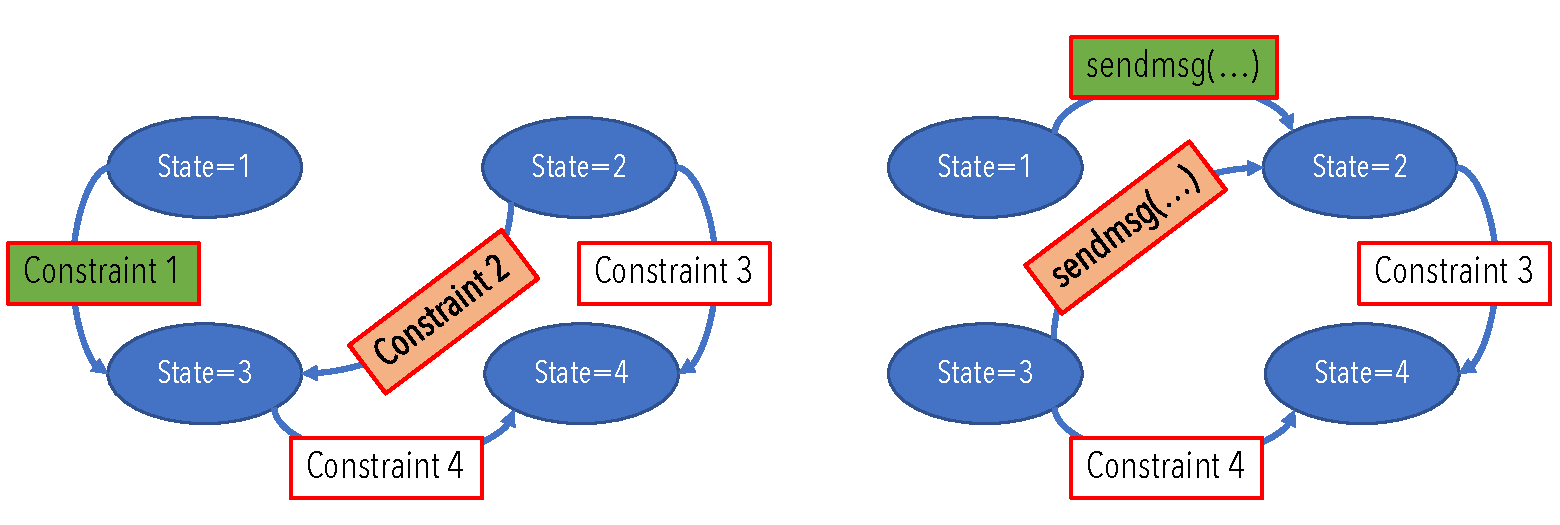
\includegraphics[width=0.47\linewidth]{figure/fsm1}\label{fig:invalid}} 
\hspace{0.05\textwidth}
\subfloat[Legitimate state machines.]{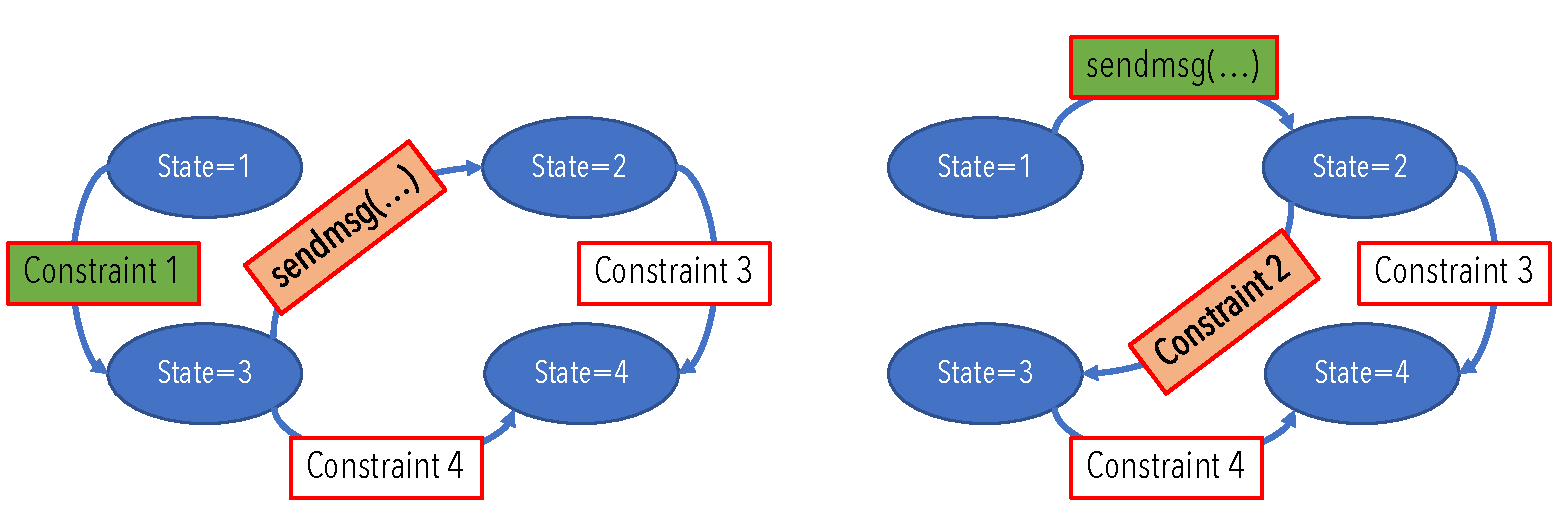
\includegraphics[width=0.47\linewidth]{figure/fsm2}\label{fig:valid}}
% \vspace{-0.1in}
\caption{Finite state machines decoupled from that indicated in Figure~\ref{fig:fsm0}.} 
\label{fig:fsm} 
\end{figure*} 

% -----------------------------------------------------------------------------

\subsubsection{Research Task 3: Constructing Finite State Machine}
\label{subsec:rt3}

With the protocol implementation and state variables identified in source code,
we now discuss how we intend to construct the state machines pertaining to the
target protocol. Since a state machine consists of not only a finite set of
states but also a series of transition conditions, we must have a mechanism to
extract the condition pertaining to each transition. In this project, we plan to
achieve this goal by performing a partial symbolic execution. To be specific, we
will first perform a breadth first search within the code fragment pertaining to
protocol implementation. With this search, we aim to identify the path tied to
each state transition. Since the constraints along a path indicates the
conditions of a possible state transition, for each path identified, we will
further perform a partial symbolic execution and record the constraint along
that path.

With the design above, we can build a transition table, where each entry carries
a pair of states as well as their transition condition. It is not difficult to
notice that we can easily construct a finite state machine using this transition
table. However, this might provide us with a state machine not truly
representing the protocol specification simply because a software developer
might implement two different protocols by sharing the same code fragment (e.g.,
the implementation of \texttt{OpenVPN}~\citep{openvpn-github}). To address this
issue, we intend to augment our protocol extraction technique with  an ability
to  decouple  state machines.

\begin{wrapfigure}{r}{0.3\textwidth}
  \centering
  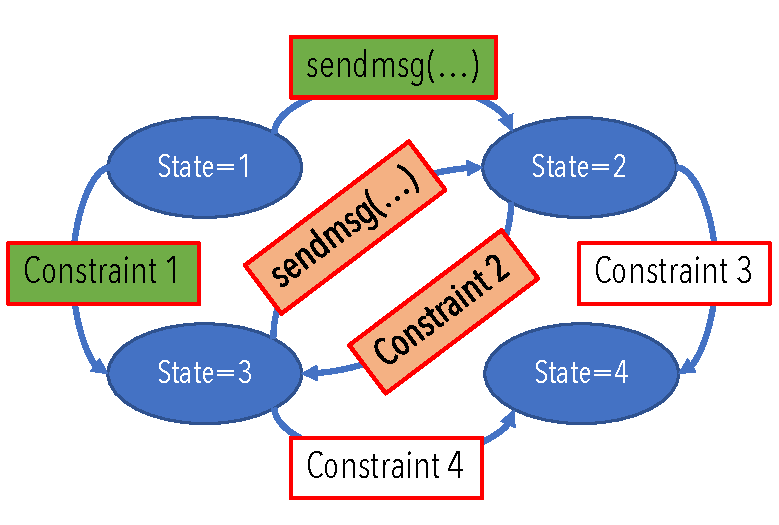
\includegraphics[width=0.3\textwidth]{figure/fsm0}
  \caption{A finite state machine carrying two independent ones.}
  \label{fig:fsm0}
\end{wrapfigure}

A finite state machine changes from one state to another in response to some
external inputs. Intuition suggests these inputs cannot be generated from the
state machine itself. Therefore, if a state machine receives a packet from
itself, it implies that the state machine extracted does not represent the
protocol specification and we must perform a state machine partition. To do it,
we plan to attach message write operations to corresponding edges on a state
machine, and then pair each of these operations with the message read. With this
design, we can decouple state machines accordingly. To illustrate this, we take
for example the state machine shown in Figure~\ref{fig:fsm0}. Assume the
rectangles in the same color indicate message read and write operations paired
together. Following the aforementioned criteria -- that a state machine cannot
receive a message sent by itself -- we can separate the state machine into four
ones as is demonstrated in Figure~\ref{fig:fsm}. From this figure, we can
observe none of these state machines decoupled involves receiving a message sent
by itself. In addition, we can observe two state machines are invalid and can be
easily eliminated because none of them includes a path along which one can
traverse all the states (see Figure~\ref{fig:invalid}). For the legitimate state
machines shown in Figure~\ref{fig:valid}, we will deem them as 
the potential finite state
machines pertaining to the target protocol.

In this project, we will explore various program analysis approaches to
implement the proposed techniques. To pair inbound and outbound messages, for
example, we can perform value set analysis against the outgoing messages prior
to its attachment to message sending, and then match that value set with the
constraints on the edges. With regard to retrieving transition conditions, we
will perform pointer analysis and build an interprocedural control flow graph
pertaining to the code fragment of the interest. Then, we will perform the
aforementioned breath first search on the graph and identify the paths
pertaining to state transitions. By modifying \texttt{KLEE} compatible with the
latest version of \texttt{LLVM}, we intend to develop a partial symbolic
execution to perform path-specific constraint extraction. Last but not least, we
will also check the constraints tied to state transitions by running constraint
solvers (\eg, \texttt{Z3} or \texttt{SMT}). This will allow us to examine the
validity of the conditions tied to transitions.

 % https://en.wikipedia.org/wiki/Finite-state_machine
% Explore the strategy of varying dialect by observing openvpn
% (1) tightening constraint on edge can remove unwanted or vulnerable component
% (2) preserving constraint on edge can also cause the change to outfacing interface
% (3) relaxing constraint is not a good idea because (1) introducing non-deterministic (2) enlarge attack surface
% (4) Add new states
% (5) Remove states through message removal
% (6) Add State though introducing new messages

\newpage

\section{Generating Various Dialects}
\label{sec:dialect}

With finite state machines extracted, we now discuss how we plan to customize a
protocol implementation to generate various dialects. To be specific, we first
discuss the challenges of protocol dialect generation. Then, we discuss how we
plan to tackle these challenges.

\subsection{Challenges}
\label{sec:task2:challenges}

Dialect generation needs to take as input a protocol implementation, and
generate various dialects. To achieve this, we have to address two major
challenges below.

\begin{wrapfigure}{r}{0.4\textwidth}
  \centering
  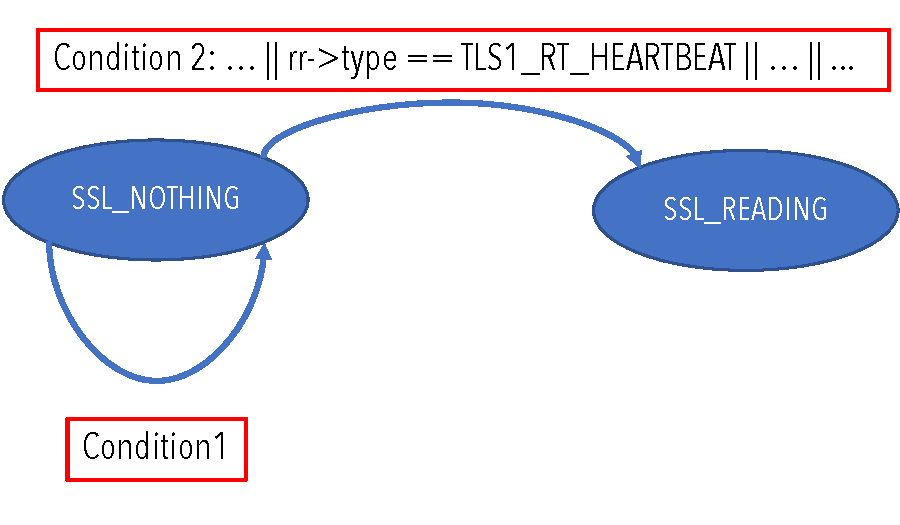
\includegraphics[width=0.4\textwidth]{figure/constraint_tighten}
  \caption{A state machine manually extracted from \texttt{OpenSSL}.}
  \label{fig:tighten}
\end{wrapfigure}

\noindent{\textbf{Recovering protocol dialects.}} The prerequisite for dialect
generation is to recover the original dialect from a protocol implementation.
To do this, an instinctive reaction is to use static analysis techniques to
identify the messages exchanging between parties. However, the research in the
past mostly focuses on performing static analysis on a single code base, and
software developers typically implement communication protocols in multiple
code bases and even involving multiple parties. As a result, our first
technical challenge for dialect generation is to design an effective approach
to restore dialects from protocol implementation.

\noindent{\textbf{Ensuring protocol validity.}}  Even though we are able to
recover dialects encoded in source code, dialect generation is still
challenging. To generate a new dialect, there are many possible strategies.
However, many of them may not guarantee the reliability (or validity) of a
dialect newly generated (\eg, generating a new dialect for \texttt{TCP}
communication by eliminating the three-way handshake). As a result, the second
challenge of dialect generation is to identify a set of effective strategies
that can generate new protocol dialects but not introduce incorrectness.

\subsection{Proposed Techniques}

In the following, we propose a series of techniques to address the challenges above. More specifically, we first introduce how we plan to recover protocol dialects using the state machines extracted. Then, we discuss how we intend to generate new valid dialects by varying state machines. 

\subsubsection{Research Task 4: Recovering Protocol Dialects}

In the context of protocol customization, it is generally challenging to achieve a clean code removal. Take the condition tightening strategy for example. As is illustrated in Figure~\ref{} and~\ref{}, we can easily pinpoint the code fragment corresponding to the removal condition. However, this is far from sufficient for clearly cutting off the code unnecessary for protocol dialects newly generated. As is mentioned in Section~\ref{sec:task2:challenges}, a communication protocol typically involves multiple parties, and a software developer may implement a protocol across different code bases and even through multiple threads. To perform a clean code removal, we must design and develop a mechanism to link all the code fragments to the one directly presented under the removal condition.  

In this project, we plan to enable this mechanism by recovering protocol dialects from implementations using the following approaches. To be specific, we will first identify the finite state machines that involve communication dialects. Since a communication dialect involves message exchanging, we intend to achieve this by examining state machines tied to function calls responsible for message sending and receiving. Second, we will pair state machines tied to the same dialect. To accomplish this, we plan to examine the data structure tied to function calls. Here, our hypothesis is that, if sending and receiving function calls are all tied to the same data structure, the corresponding state machines are involved to the same dialect. In this project, we will validate this hypothesis and if needed adjust this technique based on protocol implementations. 

After identifying and pairing state machines, we will then recover the sequence of the messages exchanged between the paired state machines. To do this, we plan to  perform value set analysis on the code base corresponding to each of the state machines. Similar to the technique proposed for refining a state machine in Section~\ref{}, we will conduct this analysis against the outgoing messages prior to its attachment to message sending, and then match that value set with transition conditions of the state machine present on the other side. To illustrate this approach, we take \texttt{OpenVPN} for example. By performing a value set analysis at the site where a client state machine sends a request message, we obtain a set of values for the message which perfectly match transition condition \Code{!(&ks->plaintext_write_buf->len) && !session->opt->server && packet.opcode == P_CONTROL_HARD_RESET_CLIENT_V2} present on the edge of a server state machine.   


With protocol dialect restored, it is not difficult to notice that one could easily pinpoint the messages exchanged between each other which can be further used for tracking down the code fragments pertaining to that of removal. For example, by tightening the condition on transition from state \texttt{S\_PRE\_START} to \texttt{S\_START} illustrated in Figure~\ref{fig:original_dialect}, we can use the dialect to pinpoint the call to that function responsible for sending \texttt{P\_ACK}. On the code base running on the client side, we can then perform backward taint and identify the code fragments relevant to message \texttt{P\_ACK} holding the removed condition. In this project, we will use the output of this backward taint to guide our code fragment removal.

\subsubsection{Research Task 5: Customizing Dialect with Transition State Variation}

\begin{wrapfigure}{r}{0.4\textwidth}
  \centering
  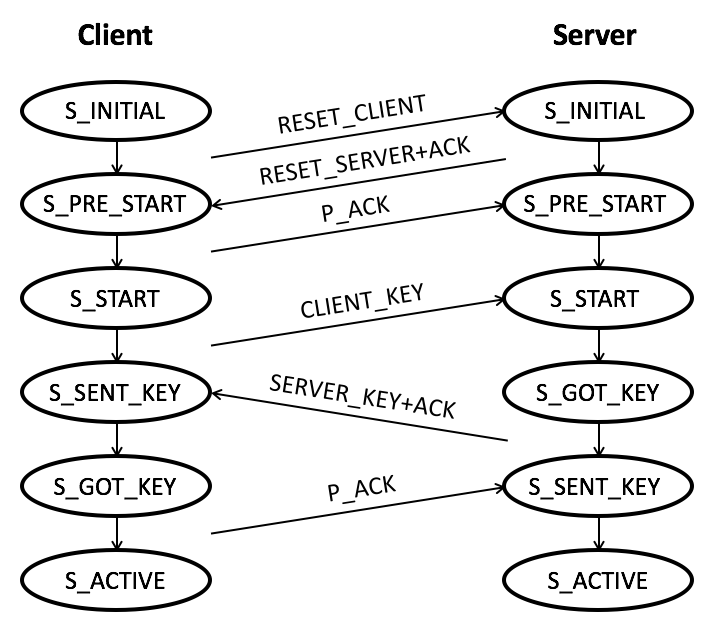
\includegraphics[width=0.4\textwidth]{figure/openvpn_protocol}
  \caption{The protocol dialects implemented in \texttt{OpenVPN} responsible for establishing a private communication tunnel. Note that the ovals indicate transition states in finite state machines extracted from a target protocol, and the edges between them demonstrate the transitions from on state to another.}
  \label{fig:original_dialect}
\end{wrapfigure}

To tackle the second challenge mentioned above, we propose two strategies to mutate transition states and thus vary dialects. In this project, we plan to develop the techniques involved and validate each of these strategies with more applications.    

{\noindent{\textbf{Eliminating states with message merging}} is our first strategy where we preserve protocol semantic by removing a state and merging the message eliminated with a consecutive message. To illustrate this, we take \texttt{OpenVPN} for example. As is shown in Figure~\ref{fig:detleted_dialect}, we first trim transition state \texttt{S\_PRE\_START} and disable the function responsible for sending message \texttt{P\_ACK}. Second, we change the target state under condition \texttt{C1} and append the information carried by \texttt{P\_ACK} to consecutive message \texttt{CLIENT\_KEY}. To be able to check message \texttt{P\_ACK} piggybacking on \texttt{CLIENT\_KEY}, we finally concatenate the transition conditions with a logic conjunction operator. In this way, we preserve the message needed for the 3-way handshake in a consecutive message. Thus, it guarantees the legitimacy of the new dialect. In this project, we will take this state elimination as \emph{the third strategy} for our dialect generation.

{\noindent{\textbf{Introducing states with message partition}} is a strategy in which we introduce not only new states but also partition messages. Again, we take \texttt{OpenVPN} for example. As is illustrated in Figure~\ref{}, on the client side, we first insert additional state \texttt{EXTRA\_CLIENT} between states \texttt{S\_PRE\_START} and \texttt{S\_START} by changing the target state under condition \texttt{C2'}. Second, we partition condition \texttt{C2'} into two individual constraints \texttt{C2.1'} and \texttt{C2.2'} so that the disjunction of these two is equivalent to \texttt{C2'} (\ie, \Code{C2.1' || C2.2' = C2'}). Third, we replace transition condition \texttt{C2'} with \texttt{C2.1'}, and introduce a new transition from state \texttt{S\_EXTRA} to state \texttt{S\_START} under condition \texttt{C2.2'}. 

Since condition \texttt{C2.1'} is the tightened version of \texttt{C2'}, and message \texttt{RESET\_SERVER+ACK} is not able to trigger the state transition from \texttt{S\_PRE\_START} to \texttt{S\_EXTRA}, we could perform a backward taint analysis from the site where the server sends message \texttt{RESET\_SERVER+ACK}. The goal of this backward taint analysis is to identify the code fragments relevant to the outgoing message \texttt{RESET\_SERVER+ACK}. With this, we will adjust the implementation based on the condition replaced, and synthesize a code snippet capable of generating a message that can trigger the transition from state \texttt{S\_EXTRA} to state \texttt{S\_START
}. In this project, we will insert this code snippet on the server into the implementation indicating the transition from state \texttt{S\_PRE\_START} to state \texttt{S\_START}. 

\subsubsection{Research Task 6: Customizing Dialect with Transition Condition Variation}

% To generate new valid dialects, we will first explore how to generate new valid dialects by varying state transitions. To be specific, 

Since a protocol dialect typically relies upon finite state machines, our study first focuses on exploring how to generate new valid dialects by varying state transitions. To be specific, we manually studied three strategies to vary transition conditions. 


\begin{wraptable}{r}{.38\textwidth}
\centering
\begin{tabular}{c}
\hspace{12pt}

\begin{lstlisting}  
else if (rr->type == TLS1_RT_HEARTBEAT) {
  dtls1_process_heartbeat(s); /* Vulnerable function */
  rr->length = 0;
  s->rwstate=SSL_READING;
  BIO_clear_retry_flags(SSL_get_rbio(s));
  BIO_set_retry_read(SSL_get_rbio(s));
  return(-1);
}
\end{lstlisting}

\end{tabular}
\caption{A code snippet under the condition eliminated vulnerable to the heartbleed bug.}
\label{code:heartbleed}
\end{wraptable} 

\noindent{\textbf{Tightening transition conditions}} is a strategy where we eliminate some conditions to tighten the constraint of triggering a state transition. To illustrate this, we take for example the state machine manually extracted from \texttt{OpenSSL} (see Figure~\ref{fig:tighten}). By removing condition \Code{rr->type == TLS1_RT_HEARTBEAT} on the state machine as well as the corresponding implementation in source code, we could tighten the condition pertaining to the transition from state \texttt{SSL\_NOTHING} to \texttt{SSL\_READING}, and cut off the heartbeat component vulnerable to the heartbleed bug~\citep{} (see Table~\ref{code:heartbleed}). Since the heartbeat component is optional for \texttt{OpenSSL}, we could obtain a new valid dialect without the heartbeat messages exchanged between a client and a server. In this project, we will take this condition tightening as \emph{the first strategy} for generating new dialects. 

\begin{wrapfigure}{r}{0.4\textwidth}
  \centering
  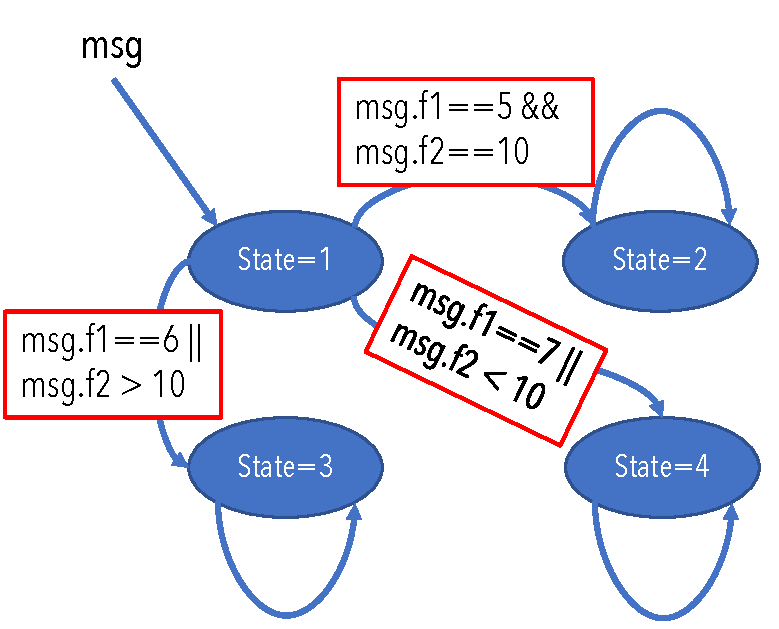
\includegraphics[width=0.4\textwidth]{figure/toy}
  \caption{A toy state machine taking as input message \texttt{msg} from a client side. Note that the constraints in the text boxes indicate transition conditions, and the message carries integer data in two fields -- \texttt{msg.f1} and \texttt{msg.f2}.}
  \label{fig:toy_fsm}
\end{wrapfigure}

\noindent{\textbf{Relaxing transition conditions}} is another strategy, in which we get rid of a condition to relax the constraint of triggering a state transition. To illustrate this, we take for example a toy protocol, a finite state machine of which is shown in Figure~\ref{fig:toy_fsm}. By getting rid of condition \Code{msg.f2==10}, we can relax the constraint pertaining to the transition from state \texttt{1} to state \texttt{2}. It is not difficult to note that such a mutation practice introduces non-deterministic to the state machine newly generated, especially when the input message holds condition \Code{msg.f1==5 && msg.f2 > 10}. As a result, we believe this transition mutation is not suitable for generating a new dialect. In this project, we will avoid performing dialect generation by following this strategy.

\begin{figure*}
  \centering
  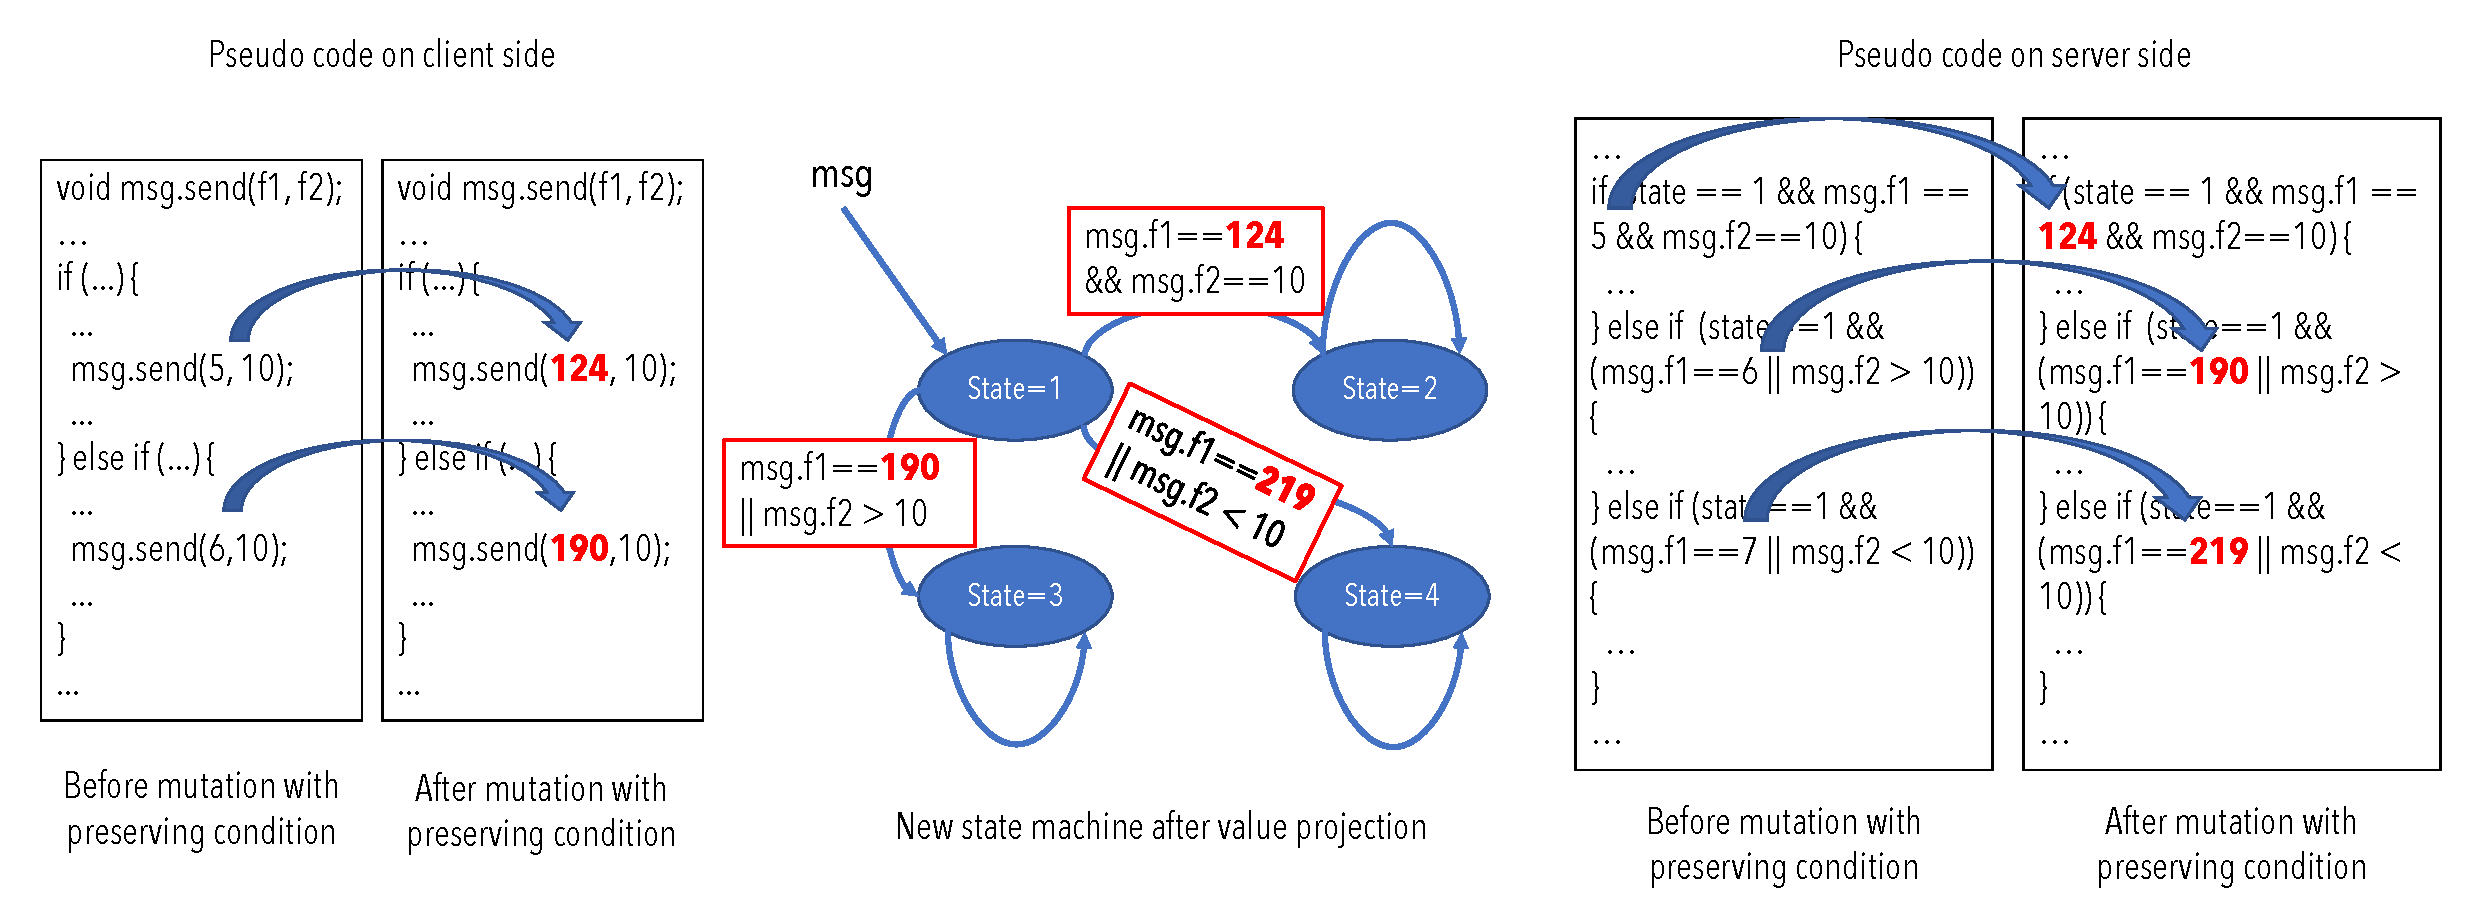
\includegraphics[width=0.95\textwidth]{figure/shuffle}
  \caption{The new state machine and pseudo code generated by following the strategy of preserving transition conditions.}
  \label{fig:toy_shuffle}
\end{figure*}

\noindent{\textbf{Preserving transition conditions}} is a strategy where we vary individual transition conditions and at the same time preserve the one indicating their combination. To illustrate this, we again take for example the state machine shown in Figure~\ref{fig:toy_fsm}. Assume \texttt{msg.f1} in condition \Code{msg.f1==5 && msg.f2==10} is an integer variable with the values from 5 to 7, indicating the operation code received from a client side. By shuffling these three values on the state machine and modifying the corresponding implementation on both ends (see Figure~\ref{fig:toy_shuffle}), we can change the state machine to a new one -- with the only difference in the state transitions -- and thus generate a new dialect in which both the client and server use new messages to coordinate the state transition. In this project, we will take this as \emph{the second strategy} for customizing protocol dialects. 





























































% \begin{figure*}[t]
% \centering
% \subfloat[Original Dialect.]{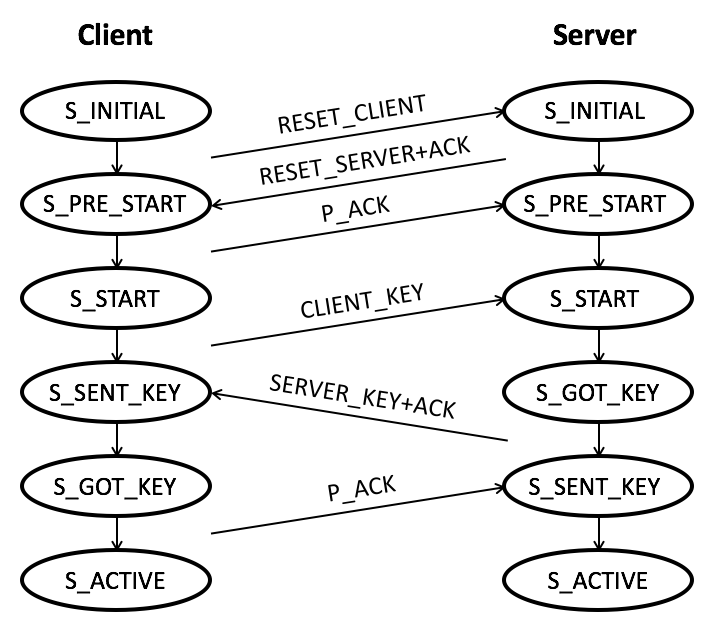
\includegraphics[width=0.33\linewidth]{figure/openvpn_protocol}\label{fig:original_dialect}} 
% \subfloat[Dialect with state removal.]{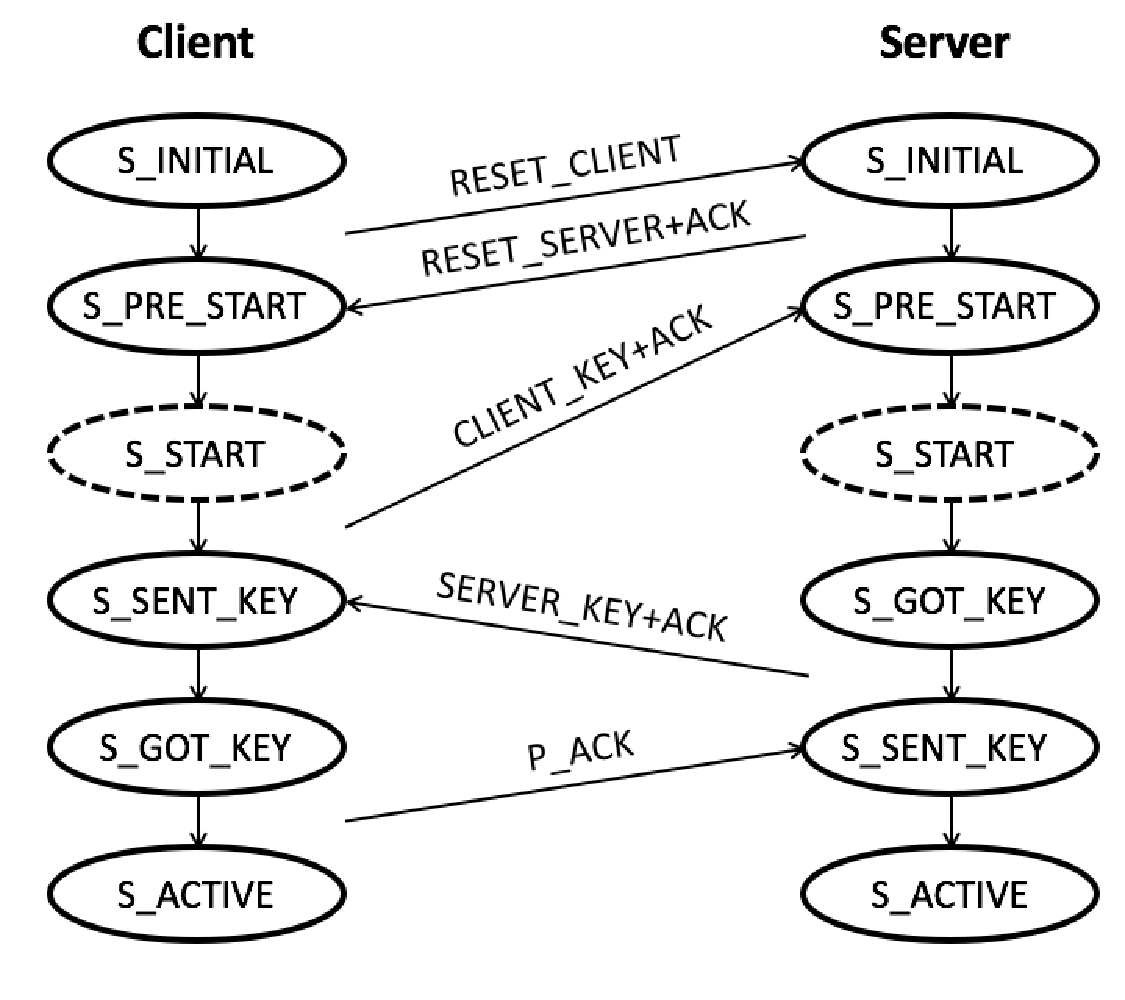
\includegraphics[width=0.33\linewidth]{figure/mutation4}\label{fig:detleted_dialect}}
% \subfloat[Dialect with state addition.]{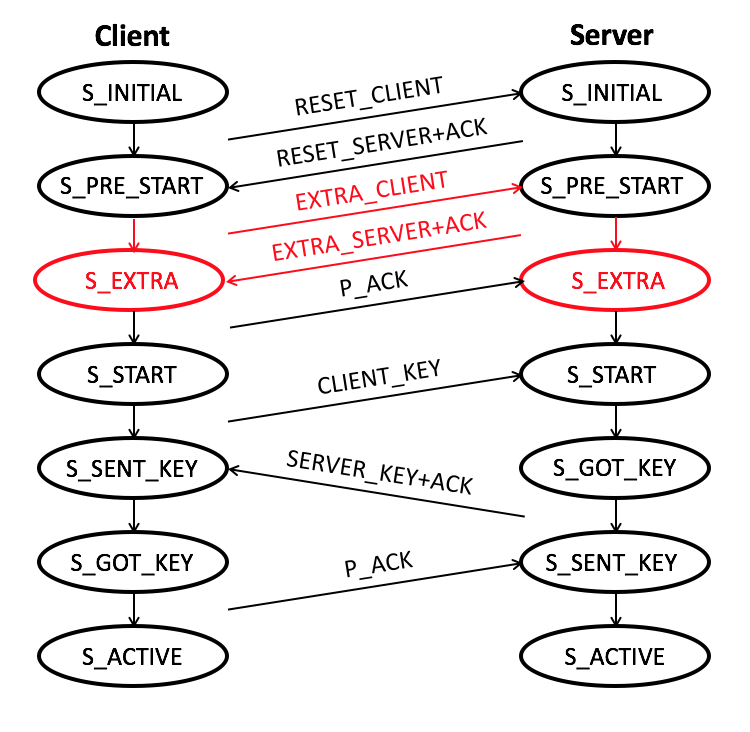
\includegraphics[width=0.33\linewidth]{figure/mutation3}\label{fig:added_dialect}} 
% \vspace{-0.1in}
% \caption{The protocol dialects implemented in \texttt{OpenVPN} responsible for establishing a private communication tunnel. Note that the ovals indicate transition states in finite state machines extracted from a target protocol, and the edges between them demonstrate the transitions from on state to another.} 
% \label{fig:dialect} 
% \end{figure*} 









% Explore the strategy of varying dialect by observing openvpn
% (1) tightening constraint on edge can remove unwanted or vulnerable component
% (2) preserving constraint on edge can also cause the change to outfacing interface
% (3) relaxing constraint is not a good idea because (1) introducing non-deterministic (2) enlarge attack surface
% (4) Add new states
% (5) Remove states through message removal
% (6) Add State though introducing new messages

% \newpage

\section{Generating Various Dialects}
\label{sec:dialect}

With finite state machines extracted, we now discuss how we plan to customize a
protocol implementation to generate various dialects. Similar to the
organization of the section above, the following discusses the challenge of
dialect generation, our preliminary exploration and the proposed techniques in
turn.


\subsection{Challenges}
\label{sec:task2:challenges}

Dialect generation needs to take as input a protocol implementation, and
generate various dialects. To achieve this, we have to address two major
challenges below.

\begin{wrapfigure}{r}{0.35\textwidth}
  \centering
  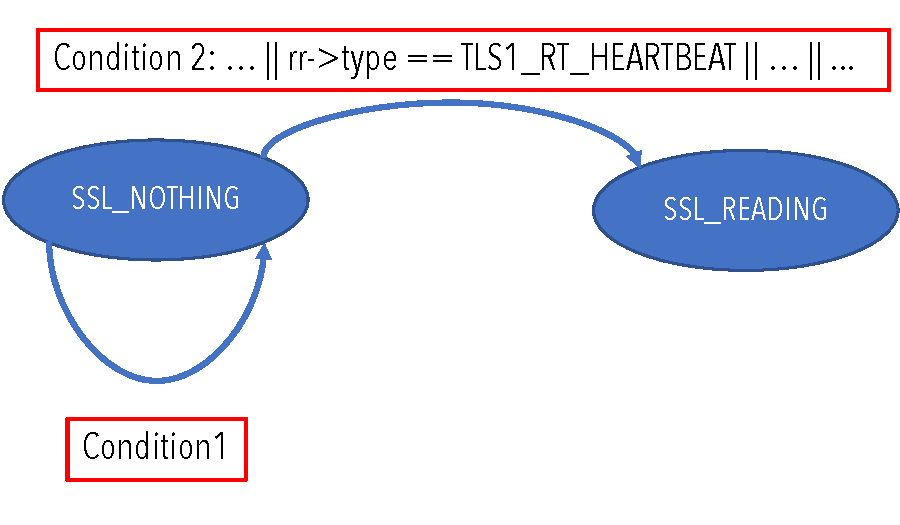
\includegraphics[width=0.3\textwidth]{figure/constraint_tighten}
  \caption{A state machine manually extracted from \texttt{OpenSSL}.}
  \label{fig:tighten}
\end{wrapfigure}

\noindent{\textbf{Validity.}}  To generate a new dialect, there are many
possible approaches. However, many of them may not guarantee the reliability (or
validity) of a dialect newly generated (\eg, generating a new dialect for
\texttt{TCP} communication by eliminating the three-way handshake). As a result,
the first challenge of dialect generation is to identify a set of effective
strategies that can generate new protocol dialects but not introduce
incorrectness.

\noindent{\textbf{Consistency.}} A communication protocol typically involves
more than one parties exchanging messages between each other. Typically, an
implementation pertaining to such a protocol are separated into different code
bases and even involved in multiple parties. When generating new dialects, we
must perform program analysis and modify a protocol implementation across
different code bases. However, research in the past mostly focuses on performing
program analysis on a single code base. Therefore, our second challenge is to
develop a set of effective techniques to perform program analysis across
different code bases and thus ensure the consistency in code variation.


\subsection{Preliminary Exploration}
\label{sec:task2:obs}

Our preliminary exploration lies in a manual study with the goal of identifying
the strategies capable of generating new and more importantly valid protocol
dialects. In the following, we describe the strategies we studied and pinpoint
those that we will use for dialect generation.

\subsubsection{Customizing Dialect with Transition Condition Variation}

Since a protocol dialect typically relies upon finite state machines, our study
first focuses on exploring how to generate new valid dialects by varying state
transitions. To be specific, we manually studied three strategies to vary
transition conditions.


\begin{wraptable}{r}{.38\textwidth}
\centering
\begin{tabular}{c}
\hspace{12pt}

\begin{lstlisting}  
else if (rr->type == TLS1_RT_HEARTBEAT) {
  dtls1_process_heartbeat(s); /* Vulnerable function */
  rr->length = 0;
  s->rwstate=SSL_READING;
  BIO_clear_retry_flags(SSL_get_rbio(s));
  BIO_set_retry_read(SSL_get_rbio(s));
  return(-1);
}
\end{lstlisting}

\end{tabular}
\caption{A code snippet under the condition eliminated vulnerable to the 
heartbleed bug.}
\label{code:heartbleed}
\end{wraptable} 

\noindent{\textbf{Tightening transition conditions}} is a strategy where we
eliminate  some conditions to tighten the constraint of triggering a state
transition. To illustrate this, we take for example the state machine manually
extracted from \texttt{OpenSSL} (see Figure~\ref{fig:tighten}). By removing
condition \Code{rr->type == TLS1_RT_HEARTBEAT} on the state machine as well as
the corresponding implementation in source code, we could tighten the condition
pertaining to the transition from state \texttt{SSL\_NOTHING} to
\texttt{SSL\_READING}, and cut off the code pertaining to the condition
eliminated. In this example, the code of removal includes the heartbeat
component vulnerable to the heartbleed bug~\citep{}, responsible for sending
heartbeat messages between the client and server (see
Table~\ref{code:heartbleed}). Therefore, we could obtain a new dialect without
the heartbeat messages. Since the heartbeat messages are optional for
\texttt{OpenSSL}, we believe this strategy is valid for generating new dialects.
In this project, we will take this condition tightening as \emph{the first
strategy} for generating new dialects.

\begin{wrapfigure}{r}{0.35\textwidth}
  \centering
  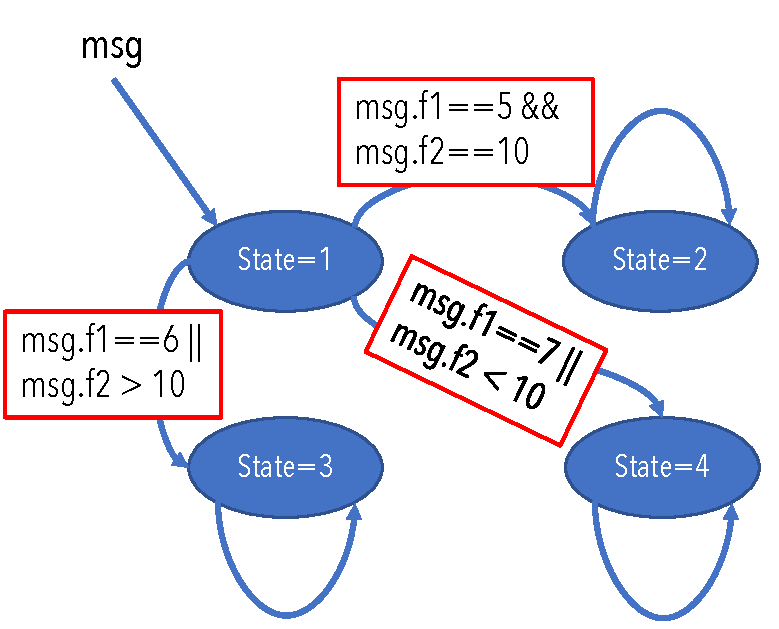
\includegraphics[width=0.3\textwidth]{figure/toy}
  \caption{A toy state machine taking as input message \texttt{msg} from a
  client side. Note that the constraints in the text boxes indicate transition
  conditions, and the message carries integer data in two fields --
  \texttt{msg.f1} and \texttt{msg.f2}.}
  \label{fig:toy_fsm}
\end{wrapfigure}

\noindent{\textbf{Relaxing transition conditions}} is another strategy,  in
which we get rid of a condition to relax the constraint of triggering a state
transition. To illustrate this, we take for example a toy protocol, a finite
state machine of which is shown in Figure~\ref{fig:toy_fsm}. By getting rid of
condition \Code{msg.f2==10}, we can relax the constraint pertaining to the
transition from state \texttt{1} to state \texttt{2}. It is not difficult to
note that such a mutation practice introduces non-deterministic to the state
machine newly generated, especially when the input message holds condition
\Code{msg.f1==5 && msg.f2 > 10}. As a result, we believe this transition
mutation is not suitable for generating a new dialect. In this project, we will
avoid performing dialect generation by following this strategy.

\begin{figure*}
  \centering
  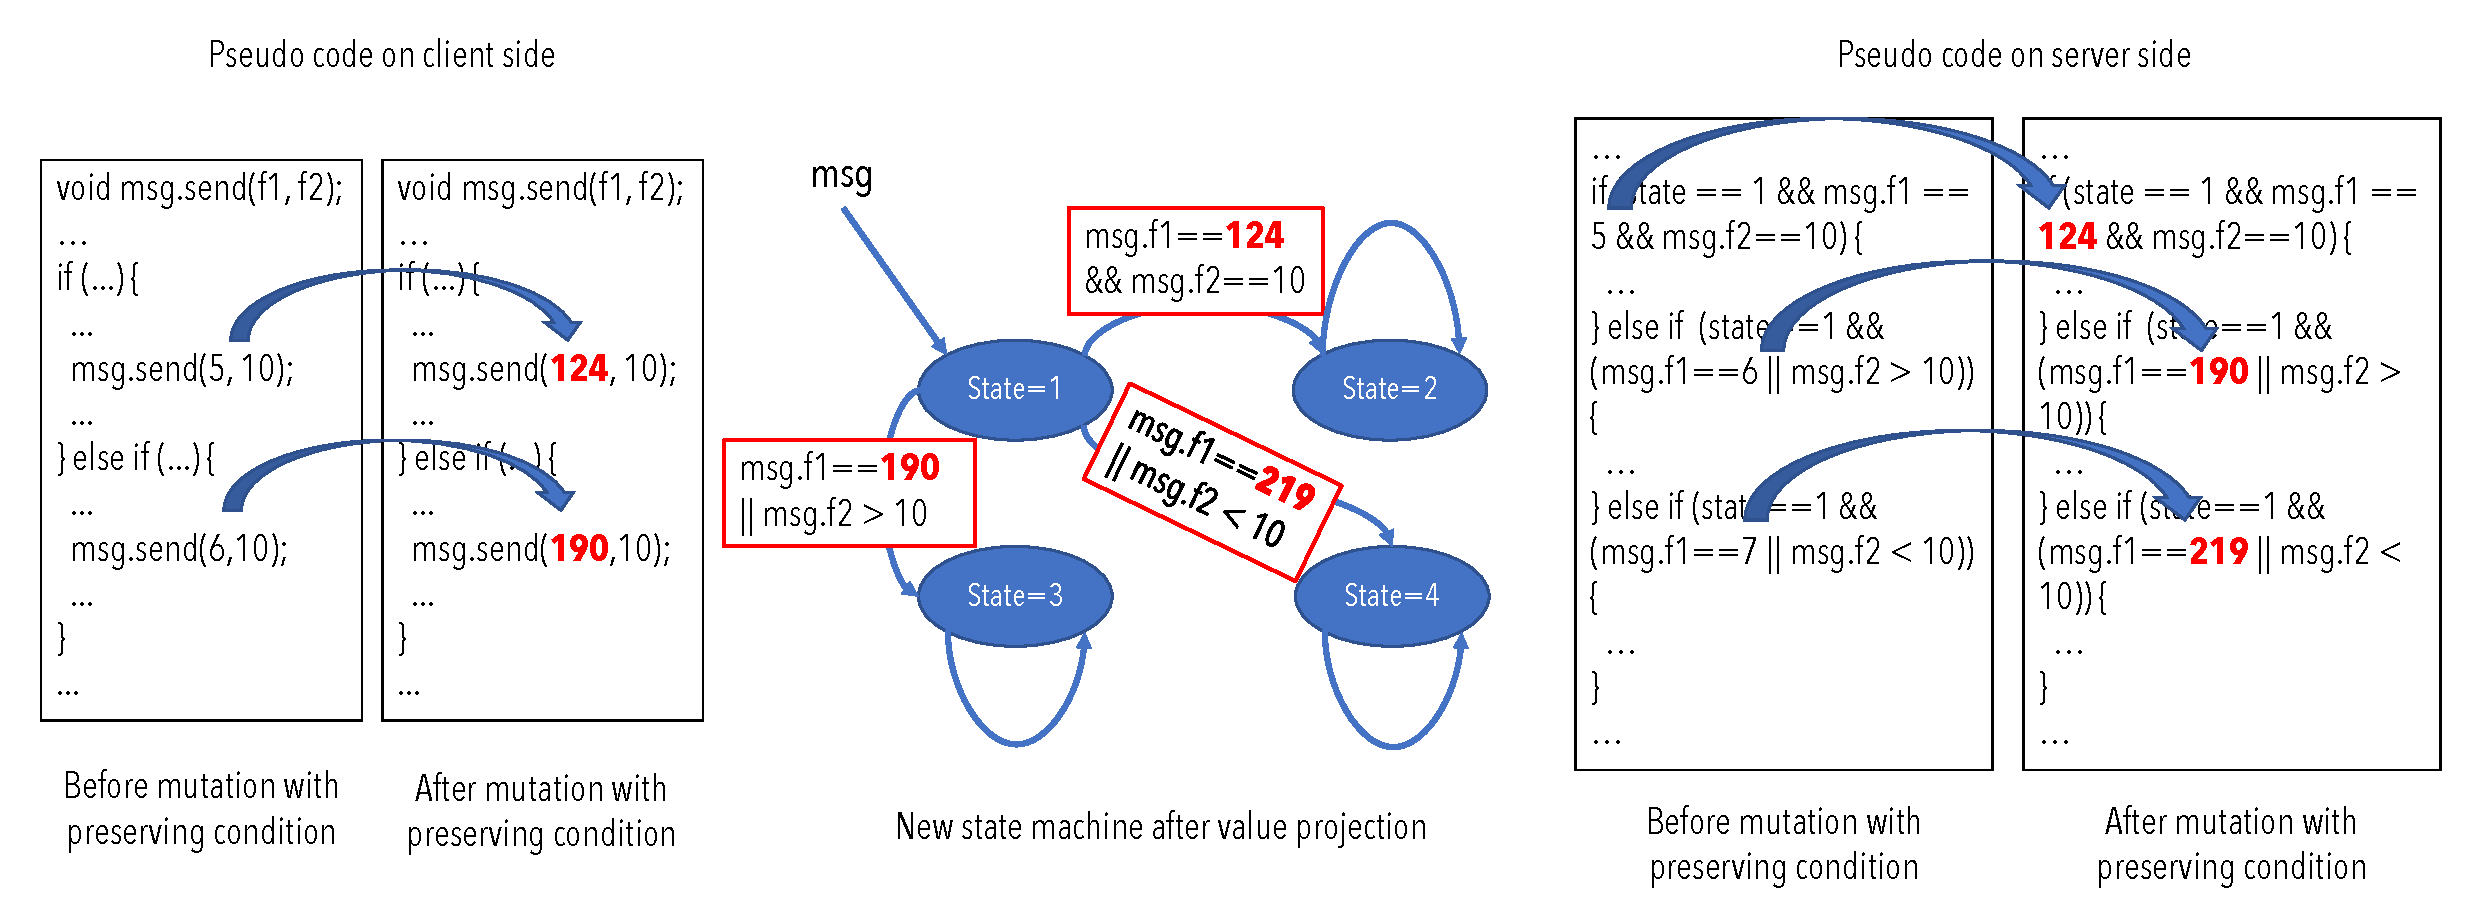
\includegraphics[width=0.95\textwidth]{figure/shuffle}
  \caption{The new state machine and pseudo code generated by following the
  strategy of preserving transition conditions.}
  \vspace{-0.1in} 
  \label{fig:toy_shuffle}
\end{figure*}

\noindent{\textbf{Preserving transition conditions}} is a strategy  where we
vary individual transition conditions and at the same time preserve the one
indicating their combination. To illustrate this, we again take for example the
state machine shown in Figure~\ref{fig:toy_fsm}. Assume \texttt{msg.f1} in
condition \Code{msg.f1==5 && msg.f2==10} is an integer variable with the values
from 5 to 7, indicating the operation code received from a client side. By
projecting these three values into new value space \texttt{(124, 190, 219)} and modifying the
corresponding implementation on both ends (see Figure~\ref{fig:toy_shuffle}), we
can change the state machine to a new one -- with the only difference in the
state transitions -- and thus generate a new dialect in which both the client
and server use new messages to coordinate the state transition. In this project,
we will take this as \emph{the second strategy} for customizing protocol
dialects.

\subsubsection{Customizing Dialect with State Variation}

To identify effective strategies for dialect generation, we also investigate how
to generate a new valid dialect by varying the transition states pertaining to
state machines extracted from a target protocol. Technically speaking, there are
many strategies to mutate transition states and vary dialects, such as deleting
and adding states. However, some practices clearly do not guarantee the
correctness of dialects newly generated. Take \texttt{OpenVPN} for example.
Figure~\ref{fig:original_dialect} illustrates a dialect of \texttt{OpenVPN} in
which the first three messages indicate a three-way handshake. By simply
removing state \texttt{S\_PRE\_START}, which further results in the elimination
of the message attached (\texttt{P\_ACK}), we can easily break the semantic of
this protocol, making message transmission unreliable. As a result, we will
avoid adding or deleting transition states in an arbitrary manner. In our
preliminary study, we have identified two strategies to perform reliable state
addition and removal. Here, we summarize both below.

\begin{wrapfigure}{r}{0.35\textwidth}
  \centering
  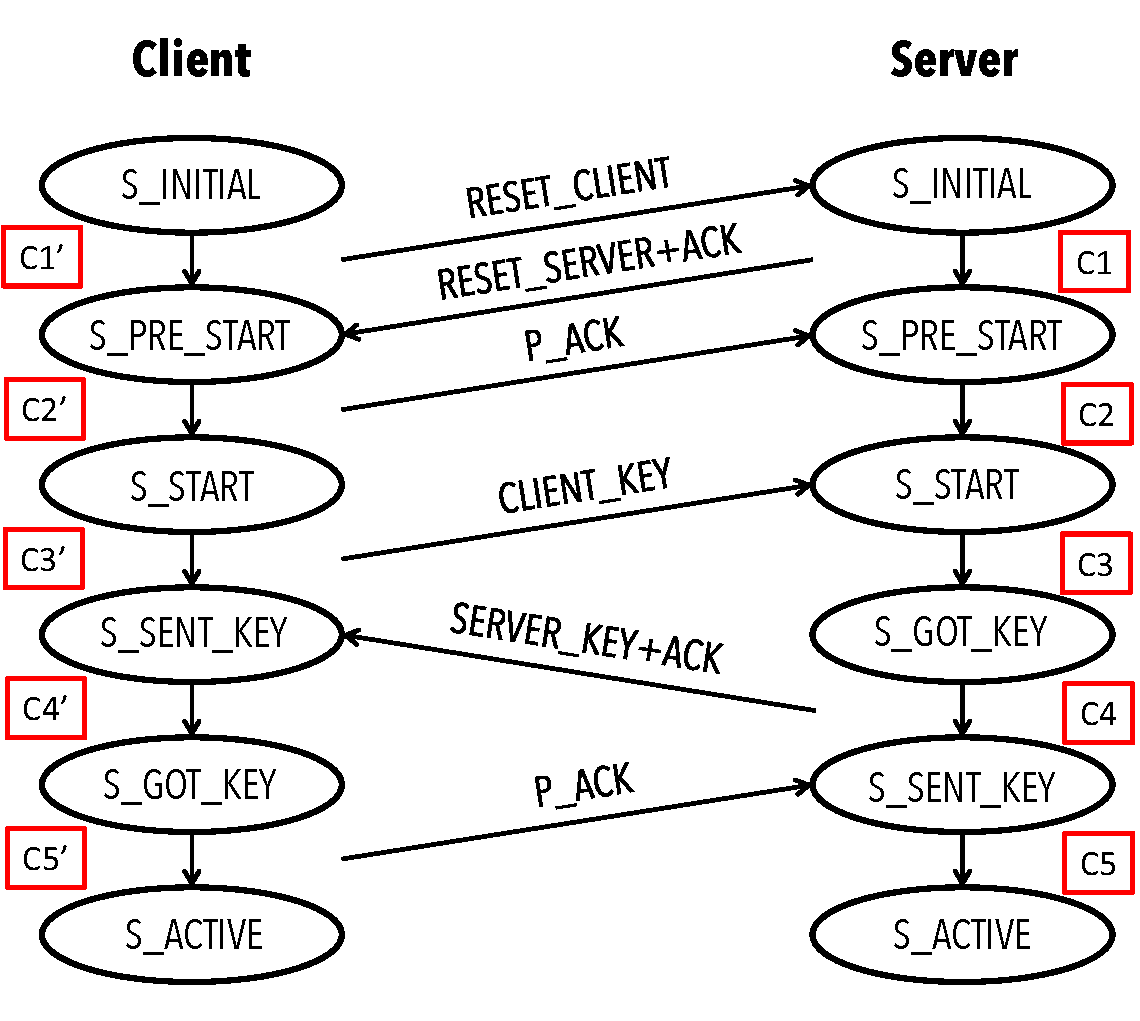
\includegraphics[width=0.3\textwidth]{figure/dialect}
  \caption{One dialect implemented in \texttt{OpenVPN} responsible for
  establishing a private communication tunnel. Note that the ovals indicate
  transition states in finite state machines extracted from \texttt{OpenVPN},
  the edges between them demonstrate the transitions from one state to another
  and the textboxes attached to the edges denote transition conditions.}  
  \label{fig:original_dialect}
\end{wrapfigure}


\begin{figure*}[t]
\centering
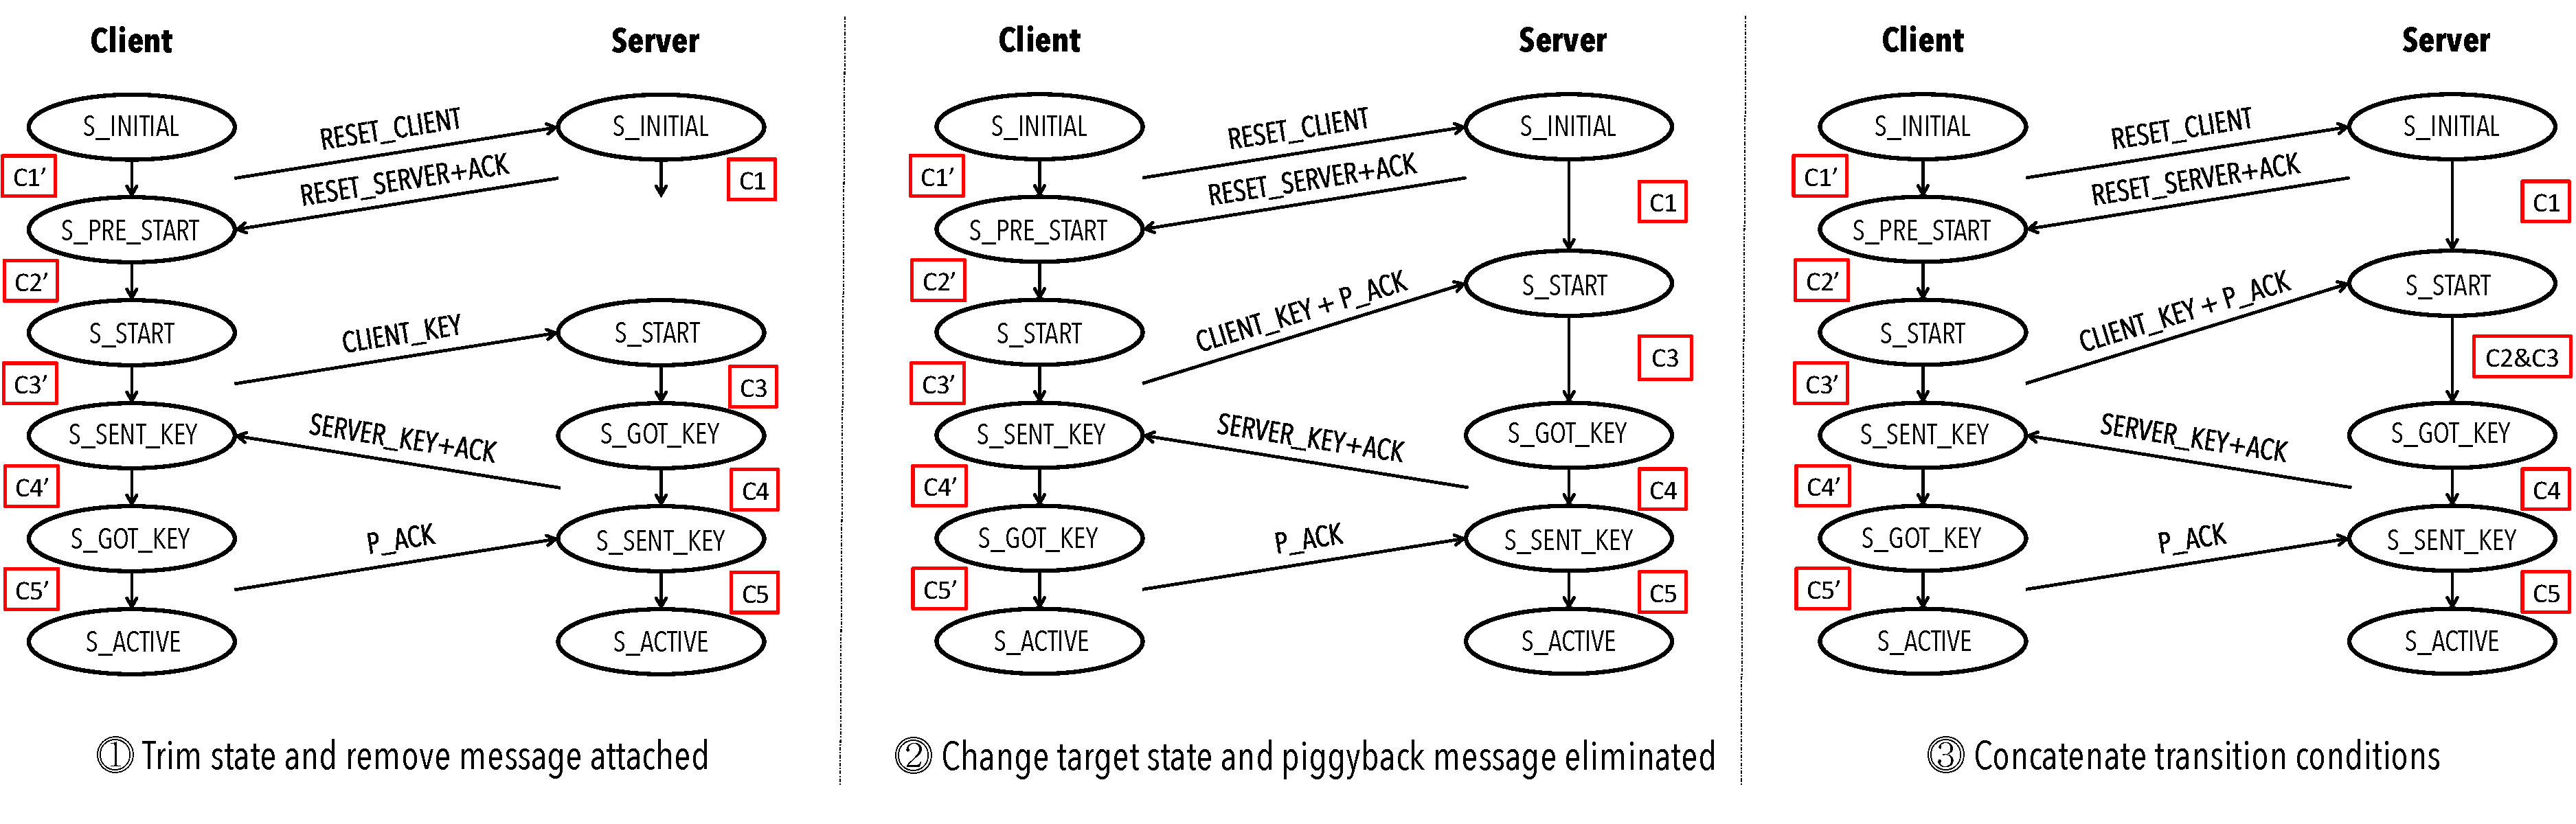
\includegraphics[width=0.95\textwidth]{figure/state_removal}
\caption{The procedure of generating a protocol dialect by removing transition 
states.} 
\vspace{-0.1in} 
\label{fig:state_removal} 
\end{figure*} 

{\noindent{\textbf{Eliminating states with message merging}} is a strategy
where we preserve protocol semantic by removing a state and merging the message
attached with a consecutive message. To illustrate this, we take
\texttt{OpenVPN} for example. As is shown in Figure~\ref{fig:state_removal}, we
first trim transition state \texttt{S\_PRE\_START} and disable the function
responsible for sending message \texttt{P\_ACK}. Second, we change the target
state under condition \texttt{C1} and append the information carried by
\texttt{P\_ACK} to consecutive message \texttt{CLIENT\_KEY}. To be able to check
message \texttt{P\_ACK} piggybacking on \texttt{CLIENT\_KEY}, we finally
concatenate the transition conditions with a logic conjunction operator. In this
way, we preserve the message needed for the 3-way handshake in a consecutive
message. Thus, it guarantees the legitimacy of the new dialect. In this project,
we will take this state elimination as \emph{the third strategy} for our dialect
generation.


\begin{figure*}[t]
\centering
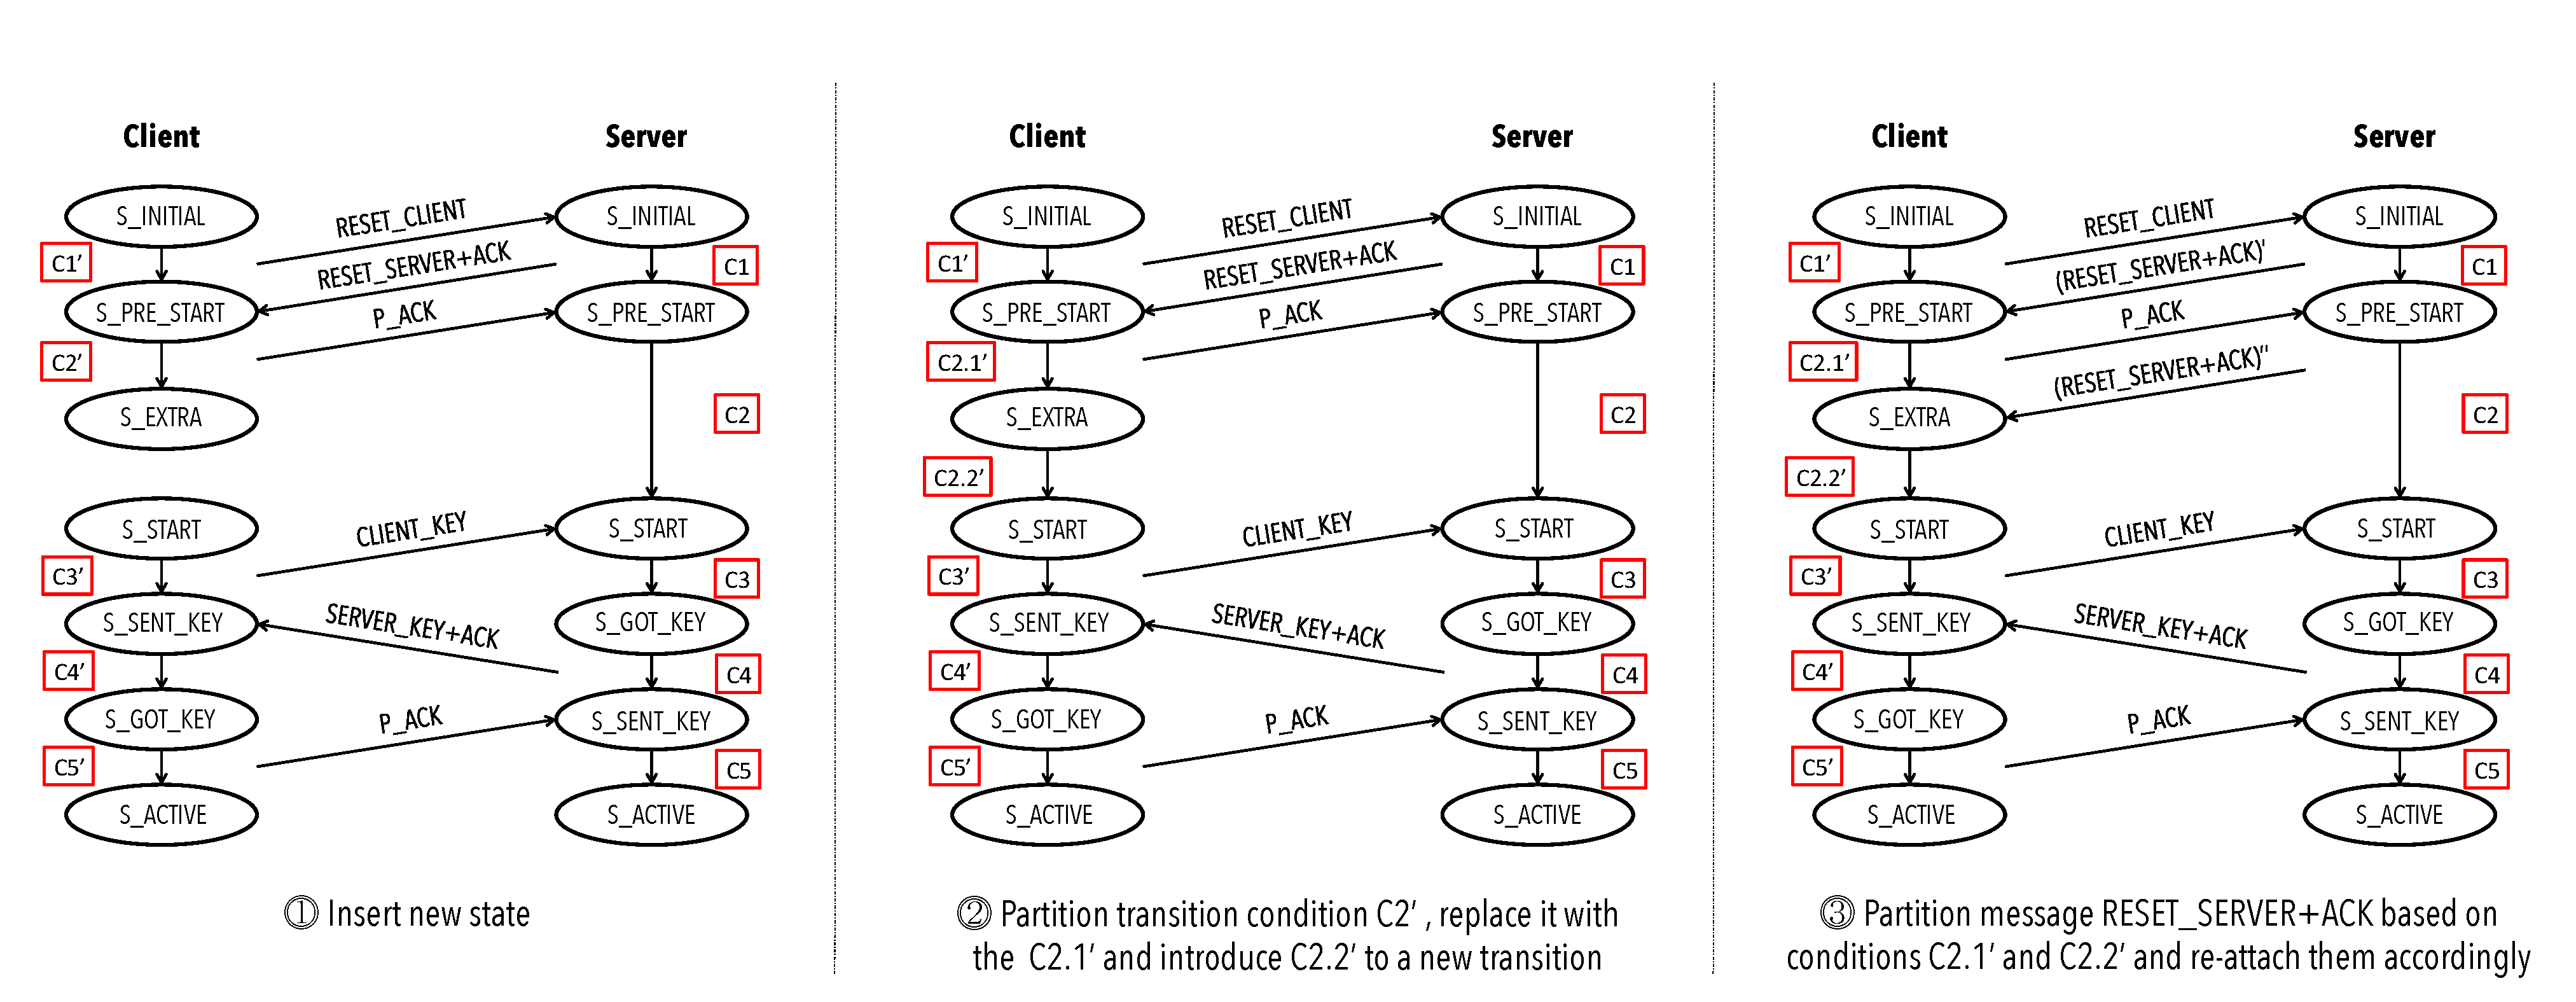
\includegraphics[width=0.95\textwidth]{figure/state_addition}
\caption{The procedure of generating a protocol dialect by introducing a new 
  transition state.} 
\vspace{-0.1in} 
\label{fig:state_addition} 
\end{figure*} 

{\noindent{\textbf{Introducing states with message partition}} is a  strategy in
which we introduce not only a new state but also partition a message. Again, we
take \texttt{OpenVPN} for example. As is shown in the first two diagrams of
Figure~\ref{fig:state_addition}, we first insert additional state
\texttt{EXTRA\_CLIENT} between states \texttt{S\_PRE\_START} and
\texttt{S\_START} by changing the target state under condition \texttt{C2'}.
Second, we partition condition \texttt{C2'} into two individual constraints
\texttt{C2.1'} and \texttt{C2.2'} so that the disjunction of these two is
equivalent to \texttt{C2'} (\ie, \Code{C2.1'||C2.2'=C2'}). Third, we replace
transition condition \texttt{C2'} with \texttt{C2.1'}, and introduce a new
transition from state \texttt{S\_EXTRA} to state \texttt{S\_START} under
condition \texttt{C2.2'}.

Since condition \texttt{C2.1'} is the tightened version of \texttt{C2'}, and
message \texttt{RESET\_SERVER+ACK} is not able to trigger the state transition
from \texttt{S\_PRE\_START} to \texttt{S\_EXTRA}, we further adjust the
implementation based on the condition replaced, and introduce a code snippet
capable of generating a message that can trigger the transition from state
\texttt{S\_EXTRA} to state \texttt{S\_START }. By inserting this code snippet
into the server code base indicating the transition from state
\texttt{S\_PRE\_START} to state \texttt{S\_START}, we construct a new dialect in
which we introduce a new state to receive the partitioned message needed for the
protocol. As we can observe from the last diagram of
Figure~\ref{fig:state_addition}, the dialect newly generated does not discard
any information. Thus, this strategy ensures the  legitimacy of the new dialect.
In this project, we will take this state elimination as \emph{the fourth
strategy} for our dialect generation.

\subsection{Proposed Techniques}

As is mentioned above, the strategies identified for dialect generation involve
code removal (\eg, tightening transition conditions requires the removal of the
code under the eliminated condition) as well as code synthesis (\eg, introducing
new transition states requires the synthesis of the code for sending out the
message partitioned). Therefore, our proposed techniques mainly focus on
designing effective code removal and synthesis mechanisms for the strategies
mentioned above.

\subsubsection{Research Task 4: Enabling Code Removal with Dialect Recovery}

In the context of protocol customization, it is generally challenging to achieve
a clean code removal. Take the condition tightening strategy for example. We can
easily pinpoint the code fragment under the removal condition. However, this is
far from sufficient because the code unnecessary for a new dialect is typically
distributed beyond the site under the condition eliminated. To address this
issue, we will design and develop a mechanism to link all the code fragments to
the one directly presented under the removal condition.

In this project, we plan to enable this mechanism by recovering protocol
dialects. To be specific, we will first identify the finite state machines that
involve communication dialects. Since a communication dialect involves message
exchanging, we intend to achieve this by examining state machines tied to
function calls responsible for message sending and receiving. Second, we will
pair state machines tied to the same dialect. To accomplish this, we plan to
examine the data structure tied to function calls. Here, our hypothesis is that,
if sending and receiving function calls are all tied to the same data structure,
the corresponding state machines are involved to the same dialect. In this
project, we will validate this hypothesis and if needed adjust this technique
based on protocol implementations.

After identifying and pairing state machines, we will then recover the sequence
of the messages exchanged between the state machines paired together. To do
this, we plan to  perform value set analysis on the code base corresponding to
each of the state machines. Similar to the technique proposed for refining a
state machine in Section~\ref{subsec:rt3}, we will conduct this analysis against
the outgoing messages prior to its attachment to message sending, and then match
that value set with transition conditions of the state machine present on the
other side. To illustrate this approach, we take \texttt{OpenVPN} for example.
By performing a value set analysis at a site where a client state machine
sends a request message, we obtain a set of values for the message which
perfectly match transition condition \Code{!(&ks->plaintext_write_buf->len) &&
!session->opt->server && packet.opcode == P_CONTROL_HARD_RESET_CLIENT_V2}
present on the edge of a server state machine.

With a protocol dialect restored, it is not difficult to notice that one could
easily pinpoint the messages exchanged between each other which can be further
used for tracking down the code fragments pertaining to that of removal. For
example, by tightening the transition condition on the server from state
\texttt{S\_PRE\_START} to \texttt{S\_START} illustrated in
Figure~\ref{fig:original_dialect}, we can use the dialect to pinpoint the call
to that function responsible for sending \texttt{P\_ACK}. On the code base
running on the client side, we can then perform backward taint and identify the
code fragments relevant to message \texttt{P\_ACK} holding the removed
condition. In this project, we will use the output of this backward taint to
guide our code fragment removal.


\subsubsection{Research Task 5: Customizing Code Synthesis Mechanisms for 
Dialect Generation Strategies}

Dialect generation strategies represent different ways to modify a protocol
implementation. For example, the first strategy mainly involves code
modification through code removal, whereas the third strategy introduces
implementation variation by adding new code and restructuring code fragments. As
a result, we must  go beyond code removal, and explore other code synthesis
mechanisms. In this project, we plan to design and develop different code
synthesis mechanisms for each of the strategies mentioned above.

For the first strategy, we will first use the aforementioned approach to
identify the code fragment relevant to the condition eliminated. Then, we will
cut off the code fragments identified, and replace the code fragment under the
removal condition with an exception handler. In this project, we will introduce
the exception handler to throw a notification while it is triggered. The reason
is that this could augment the new protocol with the ability to pinpoint the
messages that mismatch the new dialect.

For the second strategy, we will first perform value set analysis for the
variables of interest (\ie, those that we will perform value modification).
Then, we will project the set of values into a new value space. Using the
protocol dialog recovered, we will identify the site where the variables of
interest are defined, and replace the values for the variables accordingly. To
ensure the value replacement does not break the program semantic, we will
further perform a data flow analysis and if needed adjust the source code
accordingly. For example, a protocol implementation may check a condition (\eg,
\Code{if(x+y>16){...}}) which relies upon variable \texttt{x}, the value of
which has been replaced. To ensure program correctness, we need to propagate
this modification to the condition. In this project, we will explore various
approaches to achieve value projection. In addition, we will design effective
mechanisms to propagate value variations and thus achieve code modification in a
correct manner.

For the third strategy, we will first identify the code statement, indicating
the transition from predecessor states to the state of removal. From the site of
each statement identified, we will then perform a backward taint analysis to
identify the function attached to the transition responsible for receiving a
message. Using the dialog we recovered, we will trace back the message we
identified, and pinpoint the site where the function sends out the message that
we would like to piggyback. To prevent the function sending out the message, we
will remove the line of code indicating the call and introduce a buffer to hold
the message. Since the buffer we introduce will be a global variable, we could
still  retrieve the message at the site where we will perform piggybacking. In
this project, we will explore how to encode the message in the buffer into the
corresponding consecutive message.

For the last strategy, we will first extend the value set of the variable
indicating the transition state. Then, we construct an \texttt{if-else} template
based on the partitioned conditions, and perform a forward program slicing
starting from the sites of interest (\ie, the condition of partition as well as
the message we will separate). With the code sliced, we will fill in the
template, and thus synthesize the code fragments pertaining to the new
transitions. In this project, we intend to use these synthesized code fragments
as replacements for the implementation pertaining to the original transitions.


Considering the synthesis mechanisms described above may introduce
incorrectness, as part of the research project, we will also design a static
verification mechanism to identify invalid dialects. To be specific, we will
examine infeasible paths within the implementation of new state machine. By an
infeasible path, we mean a conflicting constraint along an execution path
synthesized. Throughout the project, we will explore how to leverage the output
of this verification mechanism to guide and correct our protocol dialect.






\section{Related Works}
\label{sec:related}

There are two goals to reverse engineer a protocol, 
one is to identify formats of packets exchanged through the protocol, 
and the other is to extract state machines which maintain valid sessions of the protocol. 
Existing techniques can be categorized, based on their different goals. 



\subsection{Packet Format Extraction}

To extract packet formats, 
techniques can be built based on dynamic taint analysis~\citep{AutoFormat,Polyglot,Dispatcher,ucsb-packet,wangzhi}, 
static analysis~\citep{Junghee} or analyzing network traces~\citep{Discoverer}. 

%{\textbf{\underline{Dynamic Analysis}}
{\underline{\textit{Dynamic techniques}}}
first generate execution traces using taint analysis~\citep{dawn-taint,taint1,taint-sosp,taint-micro}, 
which will mark data received from network with taint information 
and propagate this information to any instruction that operates on tainted data.
Dynamic techniques then analyze the execution traces to figure out packet formats. 
The intuition behind these techniques is that how protocol implementations 
process received packets indicates packet formats. 

Polyglot~\citep{Polyglot} models received packets in a flat structure, 
and identifies length fields, pointer fields, field separators, 
and protocol keywords through heuristics. 
~\citet{ucsb-packet} consider a untainted value as a potential delimiter, 
when the untainted value is compared with a tainted input byte, 
and label the input byte with the delimiter.
After that, a received packet will be splitted into nested intervals by delimiters, 
which represents nested fields. 
AutoFormat~\citep{AutoFormat} hierarchically identify packet fields based 
on their access contexts, such as call stacks or the addresses of instructions. 
There are many library calls and instructions whose arguments or outputs contain network semantic information, 
such as IP addresses, port numbers and timestamp.
Dispatcher~\citep{Dispatcher} leverages these system calls and 
instructions to attribute semantic information to each identified packet field. 
Dispatcher also tries to figure out fields of output packets. 
Dispatcher models an output packet as a buffer, 
which is recursively constructed from other small buffers. 
Each small buffer represents a packet field. 

{\underline{\textit{Static techniques}}} 
apply control flow and data flow analysis to infer output file or packet formats. 
FFS/x86 (File-Format Extractor for x86) uses hierarchical finite state machine (HFSM)~\citep{HFSM1, HFSM2} 
to represent output data format~\citep{Junghee,Junghee2}.
One node in HFSM represents an output library call or a callsite to a sub-FSM. 
After generating initial HFSM, 
FFS/x86 annotates each node with possible values to be written out 
and the size of the data the node represents. 
In the end, FFS/x86 simplifies HFSM by merging nodes annotated with uncertain values or sizes.
Although the idea of FFS/x86 is general, the implementation is tied to x86 instruction set. 
In their following works, TSL system~\citep{Junghee3} 
is designed to generate analyzers targeting different instruction sets. 


{\underline{\textit{Network trace analysis techniques}}}  
infer formats based on multiple collected packets. 
Discoverer~\citep{Discoverer} first breaks each packet into text tokens and binary tokens, 
and conduct initial clustering for all packets.
Tokens represent potential packet fields.
Then, Discoverer recursively splits each cluster based on 
identified format distinguisher (FD) tokens.  
FD token is a type of fields, 
which can be used to differentiate formats of subsequent parts. 
Finally, Discoverer will merge similar clusters to eliminate cases, 
where packets of the same format are classified into different clusters. 
Tupni~\citep{Tupni} combines dynamic taint analysis and trace analysis. 
After generating packet format for every packet, 
Tupni will merge all packet formats to drive a more complete specification. 

Although techniques to extract packet formats are useful in guiding black-box fuzzing, 
deep packet inspection and packet rewriting, 
they do not identify protocols’ state machines and cannot provide any guidance 
in protocol subsetting and dialect generation. 


\subsection{Protocol State Machine Extraction}

Existing techniques~\citep{botnet-inference,MACE,Prospex} extract state machines through analyzing network traffics in two steps.
First, these techniques apply an abstract function to change concrete packets into a set of abstract messages.
Second, L* algorithm~\citep{L1,L2}  is applied on network traffics represented by abstract messages to generate state machines.   

L* is an online algorithm~\citep{L1,L2} to infer a finite state machine 
based on queries to the finite state machine and its responses. 
L* assumes the finite state machine to be inferred will answer queries in a deterministic way. 
It also assumes that there is an oracle which will tell whether the current learned state machine is equivalent to the real one.
If not, the oracle will generate a counterexample, which L* can use to continue the inference process. 
The complexity of L* is polynomial in the number of states and the size of input alphabet. 


~\citet{botnet-inference} design several optimizations when applying L* algorithm, 
such as parallelization and caching, and also demonstrate that 
inferred state machines can be used as a formal basis to study and defeat botnet
such as identifying the weakest link in a botnet protocol and proving the existence 
of communication channels between botnet masters.  
MACE~\citep{MACE} incrementally infers state machines by combining 
L* algorithm and concolic exploration~\citep{dart,cute}. 
In each iteration, MACE use a sequence of input packets to make the monitored protocol 
implementation get to a known state, and then use concolic execution to explore new states.  
Compared with concolic execution, MACE is less likely to be stuck in local state sub-spaces. 
Prospex~\citep{Prospex} starts state machine inference from clustering packets, 
based on packet field similarity, execution similarity and output similarity. 
Then, Prospex leverage an abstract function to assign a type to each cluster. 
A session can be represented as a sequence of packet types. 
L* algorithm is applied to infer a state machine which can take the sequence as input. 

Although these techniques are useful, 
they largely treat analyzed protocol implementation as a black box, 
and their identified protocol states and message types 
do not correspond to specific codes in the protocol implementation.
Therefore, extracted state machines cannot provide any guidance for protocol subsetting and dialect generation. 
Since all these techniques are based on collected network traces, 
which may not cover all protocol states, 
they cannot guarantee inferred state machines are complete. 


%%\balance
%\begin{spacing}{0.65}

\balance
{
\bibliographystyle{abbrvnat}
\bibliography{security} 
}
%\end{spacing}
\end{document}
